%% Manuscript for Computational Statistics (Springer).
%% Compile with the Springer Nature LaTeX template (sn-jnl.cls), e.g. in the
%% Overleaf "Springer Nature LaTeX Template" project: upload this file, refs.bib,
%% numbers.tex, tables/ and figures/ (no subfolders are required by the journal:
%% see README_SUBMISSION_TR.md for flattening). Numbers come from numbers.tex and
%% tables/*.tex, which are generated by analysis/make_tables.py.

\documentclass[pdflatex,sn-mathphys-ay]{sn-jnl}

\usepackage{graphicx}
\usepackage{multirow}
\usepackage{amsmath,amssymb,amsfonts}
\usepackage{amsthm}
\usepackage{booktabs}
\usepackage{xcolor}
\usepackage{textcomp}
\usepackage{url}

\theoremstyle{thmstyleone}
\newtheorem{proposition}{Proposition}
\theoremstyle{thmstylethree}
\newtheorem{remark}{Remark}

\raggedbottom

% Generated by analysis/make_tables.py from analysis/out; do not edit by hand.
\newcommand{\NDecisions}{72}
\newcommand{\NBoot}{2,000}
\newcommand{\NRecompute}{1,120}
\newcommand{\RecomputeMaxDiff}{\ensuremath{1.7\times 10^{-16}}}
\newcommand{\BalQwk}{0.72}
\newcommand{\RegEndQwk}{0.55}
\newcommand{\RegQwkQwk}{0.06}
\newcommand{\RegMaeQwk}{0.48}
\newcommand{\RegMmaeQwk}{0.29}
\newcommand{\RankEndQwk}{4.08}
\newcommand{\RankQwkQwk}{2.25}
\newcommand{\AgrQwkQwk}{1.00}
\newcommand{\AgrQwkMae}{0.22}
\newcommand{\AgrQwkAmae}{0.53}
\newcommand{\AgrQwkMmae}{0.47}
\newcommand{\AgrQwkMfone}{0.79}
\newcommand{\AgrQwkRps}{0.18}
\newcommand{\AgrQwkCon}{0.56}
\newcommand{\BalMae}{0.00}
\newcommand{\RegEndMae}{0.89}
\newcommand{\RegQwkMae}{0.55}
\newcommand{\RegMaeMae}{0.01}
\newcommand{\RegMmaeMae}{0.91}
\newcommand{\RankEndMae}{5.58}
\newcommand{\RankQwkMae}{4.75}
\newcommand{\AgrMaeQwk}{0.22}
\newcommand{\AgrMaeMae}{1.00}
\newcommand{\AgrMaeAmae}{0.19}
\newcommand{\AgrMaeMmae}{0.01}
\newcommand{\AgrMaeMfone}{0.18}
\newcommand{\AgrMaeRps}{0.68}
\newcommand{\AgrMaeCon}{0.00}
\newcommand{\BalAmae}{0.68}
\newcommand{\RegEndAmae}{0.48}
\newcommand{\RegQwkAmae}{0.35}
\newcommand{\RegMaeAmae}{0.56}
\newcommand{\RegMmaeAmae}{0.42}
\newcommand{\RankEndAmae}{4.04}
\newcommand{\RankQwkAmae}{3.92}
\newcommand{\AgrAmaeQwk}{0.53}
\newcommand{\AgrAmaeMae}{0.19}
\newcommand{\AgrAmaeAmae}{1.00}
\newcommand{\AgrAmaeMmae}{0.43}
\newcommand{\AgrAmaeMfone}{0.51}
\newcommand{\AgrAmaeRps}{0.14}
\newcommand{\AgrAmaeCon}{0.57}
\newcommand{\BalMmae}{0.93}
\newcommand{\RegEndMmae}{0.29}
\newcommand{\RegQwkMmae}{0.36}
\newcommand{\RegMaeMmae}{0.78}
\newcommand{\RegMmaeMmae}{0.06}
\newcommand{\RankEndMmae}{2.29}
\newcommand{\RankQwkMmae}{4.79}
\newcommand{\AgrMmaeQwk}{0.47}
\newcommand{\AgrMmaeMae}{0.01}
\newcommand{\AgrMmaeAmae}{0.43}
\newcommand{\AgrMmaeMmae}{1.00}
\newcommand{\AgrMmaeMfone}{0.32}
\newcommand{\AgrMmaeRps}{0.01}
\newcommand{\AgrMmaeCon}{0.67}
\newcommand{\BalMfone}{0.72}
\newcommand{\RegEndMfone}{0.52}
\newcommand{\RegQwkMfone}{0.07}
\newcommand{\RegMaeMfone}{0.50}
\newcommand{\RegMmaeMfone}{0.27}
\newcommand{\RankEndMfone}{4.04}
\newcommand{\RankQwkMfone}{3.04}
\newcommand{\AgrMfoneQwk}{0.79}
\newcommand{\AgrMfoneMae}{0.18}
\newcommand{\AgrMfoneAmae}{0.51}
\newcommand{\AgrMfoneMmae}{0.32}
\newcommand{\AgrMfoneMfone}{1.00}
\newcommand{\AgrMfoneRps}{0.15}
\newcommand{\AgrMfoneCon}{0.43}
\newcommand{\BalRps}{0.00}
\newcommand{\RegEndRps}{0.81}
\newcommand{\RegQwkRps}{0.56}
\newcommand{\RegMaeRps}{0.02}
\newcommand{\RegMmaeRps}{0.91}
\newcommand{\RankEndRps}{5.38}
\newcommand{\RankQwkRps}{4.75}
\newcommand{\AgrRpsQwk}{0.18}
\newcommand{\AgrRpsMae}{0.68}
\newcommand{\AgrRpsAmae}{0.14}
\newcommand{\AgrRpsMmae}{0.01}
\newcommand{\AgrRpsMfone}{0.15}
\newcommand{\AgrRpsRps}{1.00}
\newcommand{\AgrRpsCon}{0.00}
\newcommand{\BalCon}{0.99}
\newcommand{\RegEndCon}{0.25}
\newcommand{\RegQwkCon}{0.40}
\newcommand{\RegMaeCon}{0.85}
\newcommand{\RegMmaeCon}{0.09}
\newcommand{\RankEndCon}{2.58}
\newcommand{\RankQwkCon}{4.50}
\newcommand{\AgrConQwk}{0.56}
\newcommand{\AgrConMae}{0.00}
\newcommand{\AgrConAmae}{0.57}
\newcommand{\AgrConMmae}{0.67}
\newcommand{\AgrConMfone}{0.43}
\newcommand{\AgrConRps}{0.00}
\newcommand{\AgrConCon}{1.00}
\newcommand{\RegOwnMax}{0.11}
\newcommand{\FriedEndChi}{26.4}
\newcommand{\FriedEndP}{\ensuremath{<}0.001}
\newcommand{\FriedQwkChi}{16.3}
\newcommand{\FriedQwkP}{\ensuremath{=}0.012}
\newcommand{\NemenyiCD}{2.60}
\newcommand{\WilPAmae}{0.820}
\newcommand{\WilPosAmae}{3}
\newcommand{\WilNegAmae}{6}
\newcommand{\WilMedAmae}{\ensuremath{-}0.003}
\newcommand{\WilMeanAmae}{\ensuremath{+}0.004}
\newcommand{\QwkCostMedAmae}{\ensuremath{-}0.009}
\newcommand{\QwkCostNegAmae}{7}
\newcommand{\QwkCostPAmae}{0.039}
\newcommand{\WilPMfone}{0.938}
\newcommand{\WilPosMfone}{4}
\newcommand{\WilNegMfone}{3}
\newcommand{\WilMedMfone}{0.000}
\newcommand{\WilMeanMfone}{\ensuremath{+}0.004}
\newcommand{\QwkCostMedMfone}{0.000}
\newcommand{\QwkCostNegMfone}{7}
\newcommand{\QwkCostPMfone}{0.195}
\newcommand{\WilPCon}{0.031}
\newcommand{\WilPosCon}{6}
\newcommand{\WilNegCon}{0}
\newcommand{\WilMedCon}{\ensuremath{+}0.024}
\newcommand{\WilMeanCon}{\ensuremath{+}0.086}
\newcommand{\QwkCostMedCon}{\ensuremath{-}0.020}
\newcommand{\QwkCostNegCon}{6}
\newcommand{\QwkCostPCon}{0.031}
\newcommand{\WilPMmae}{0.039}
\newcommand{\WilPosMmae}{7}
\newcommand{\WilNegMmae}{1}
\newcommand{\WilMedMmae}{\ensuremath{+}0.002}
\newcommand{\WilMeanMmae}{\ensuremath{+}0.050}
\newcommand{\QwkCostMedMmae}{\ensuremath{-}0.010}
\newcommand{\QwkCostNegMmae}{8}
\newcommand{\QwkCostPMmae}{0.012}
\newcommand{\WilPMae}{0.055}
\newcommand{\WilPosMae}{2}
\newcommand{\WilNegMae}{7}
\newcommand{\WilMedMae}{\ensuremath{-}0.040}
\newcommand{\WilMeanMae}{\ensuremath{-}0.141}
\newcommand{\QwkCostMedMae}{\ensuremath{-}0.042}
\newcommand{\QwkCostNegMae}{8}
\newcommand{\QwkCostPMae}{0.020}
\newcommand{\WilPRps}{0.055}
\newcommand{\WilPosRps}{2}
\newcommand{\WilNegRps}{7}
\newcommand{\WilMedRps}{\ensuremath{-}0.034}
\newcommand{\WilMeanRps}{\ensuremath{-}0.129}
\newcommand{\QwkCostMedRps}{\ensuremath{-}0.039}
\newcommand{\QwkCostNegRps}{8}
\newcommand{\QwkCostPRps}{0.027}
\newcommand{\HolmCon}{0.094}
\newcommand{\AmaeMin}{\ensuremath{-}0.40}
\newcommand{\AmaeMax}{\ensuremath{+}0.53}
\newcommand{\ConQwkMedCell}{\ensuremath{-}0.020}
\newcommand{\ModRho}{\ensuremath{-}0.64}
\newcommand{\ModP}{0.026}
\newcommand{\ModCells}{12}
\newcommand{\CtrlPosEnd}{21}
\newcommand{\CtrlNegEnd}{3}
\newcommand{\CtrlMedEnd}{\ensuremath{+}0.145}
\newcommand{\CtrlPosMae}{24}
\newcommand{\CtrlNegMae}{0}
\newcommand{\CtrlMedMae}{\ensuremath{+}0.083}
\newcommand{\CtrlPosMmae}{2}
\newcommand{\CtrlNegMmae}{22}
\newcommand{\CtrlMedMmae}{\ensuremath{-}0.204}
\newcommand{\CtrlPosQwk}{17}
\newcommand{\CtrlNegQwk}{7}
\newcommand{\CtrlMedQwk}{\ensuremath{+}0.020}
\newcommand{\CtrlPosLow}{23}
\newcommand{\CtrlNegLow}{0}
\newcommand{\CtrlMedLow}{\ensuremath{+}0.320}
\newcommand{\CtrlPosHigh}{15}
\newcommand{\CtrlNegHigh}{8}
\newcommand{\CtrlMedHigh}{\ensuremath{+}0.121}
\newcommand{\CtrlPosAmae}{9}
\newcommand{\CtrlNegAmae}{15}
\newcommand{\CtrlMedAmae}{\ensuremath{-}0.020}
\newcommand{\CtrlN}{24}
\newcommand{\ConFallbacks}{14}
\newcommand{\ConFallbacksWine}{14}
\newcommand{\PredVarMlPoQwk}{2.68}
\newcommand{\EndShareMlPoQwk}{0.60}
\newcommand{\LowMlPoQwk}{0.52}
\newcommand{\HighMlPoQwk}{0.40}
\newcommand{\ObsMlPoQwk}{3.44}
\newcommand{\ExpMlPoQwk}{4.28}
\newcommand{\QwkMlPoQwk}{0.196}
\newcommand{\NamaeMlPoQwk}{0.354}
\newcommand{\NmmaeMlPoQwk}{0.388}
\newcommand{\PredVarMlPoAmae}{0.23}
\newcommand{\EndShareMlPoAmae}{0.06}
\newcommand{\LowMlPoAmae}{0.00}
\newcommand{\HighMlPoAmae}{0.11}
\newcommand{\ObsMlPoAmae}{1.41}
\newcommand{\ExpMlPoAmae}{1.63}
\newcommand{\QwkMlPoAmae}{0.137}
\newcommand{\NamaeMlPoAmae}{0.323}
\newcommand{\NmmaeMlPoAmae}{0.669}
\newcommand{\LabVarMl}{1.28}
\newcommand{\LabEndMl}{0.28}
\newcommand{\PredVarMlRfQwk}{1.98}
\newcommand{\EndShareMlRfQwk}{0.41}
\newcommand{\LowMlRfQwk}{0.26}
\newcommand{\HighMlRfQwk}{0.38}
\newcommand{\ObsMlRfQwk}{2.65}
\newcommand{\ExpMlRfQwk}{3.36}
\newcommand{\QwkMlRfQwk}{0.211}
\newcommand{\NamaeMlRfQwk}{0.326}
\newcommand{\NmmaeMlRfQwk}{0.399}
\newcommand{\PredVarMlRfAmae}{1.27}
\newcommand{\EndShareMlRfAmae}{0.28}
\newcommand{\LowMlRfAmae}{0.14}
\newcommand{\HighMlRfAmae}{0.32}
\newcommand{\ObsMlRfAmae}{2.04}
\newcommand{\ExpMlRfAmae}{2.55}
\newcommand{\QwkMlRfAmae}{0.202}
\newcommand{\NamaeMlRfAmae}{0.321}
\newcommand{\NmmaeMlRfAmae}{0.527}
\newcommand{\PredVarWrPoQwk}{0.37}
\newcommand{\EndShareWrPoQwk}{0.00}
\newcommand{\LowWrPoQwk}{0.00}
\newcommand{\HighWrPoQwk}{0.00}
\newcommand{\ObsWrPoQwk}{0.51}
\newcommand{\ExpWrPoQwk}{1.03}
\newcommand{\QwkWrPoQwk}{0.502}
\newcommand{\NamaeWrPoQwk}{0.212}
\newcommand{\NmmaeWrPoQwk}{0.410}
\newcommand{\PredVarWrPoAmae}{1.92}
\newcommand{\EndShareWrPoAmae}{0.16}
\newcommand{\LowWrPoAmae}{0.45}
\newcommand{\HighWrPoAmae}{0.61}
\newcommand{\ObsWrPoAmae}{1.37}
\newcommand{\ExpWrPoAmae}{2.58}
\newcommand{\QwkWrPoAmae}{0.469}
\newcommand{\NamaeWrPoAmae}{0.154}
\newcommand{\NmmaeWrPoAmae}{0.193}
\newcommand{\LabVarWr}{0.65}
\newcommand{\LabEndWr}{0.02}
\newcommand{\PredVarWrRfQwk}{0.80}
\newcommand{\EndShareWrRfQwk}{0.02}
\newcommand{\LowWrRfQwk}{0.00}
\newcommand{\HighWrRfQwk}{0.06}
\newcommand{\ObsWrRfQwk}{0.67}
\newcommand{\ExpWrRfQwk}{1.45}
\newcommand{\QwkWrRfQwk}{0.541}
\newcommand{\NamaeWrRfQwk}{0.173}
\newcommand{\NmmaeWrRfQwk}{0.320}
\newcommand{\PredVarWrRfAmae}{1.36}
\newcommand{\EndShareWrRfAmae}{0.07}
\newcommand{\LowWrRfAmae}{0.05}
\newcommand{\HighWrRfAmae}{0.22}
\newcommand{\ObsWrRfAmae}{1.04}
\newcommand{\ExpWrRfAmae}{2.01}
\newcommand{\QwkWrRfAmae}{0.484}
\newcommand{\NamaeWrRfAmae}{0.168}
\newcommand{\NmmaeWrRfAmae}{0.270}
\newcommand{\PredVarScPoQwk}{2.73}
\newcommand{\EndShareScPoQwk}{0.14}
\newcommand{\LowScPoQwk}{0.56}
\newcommand{\HighScPoQwk}{0.70}
\newcommand{\ObsScPoQwk}{1.32}
\newcommand{\ExpScPoQwk}{4.83}
\newcommand{\QwkScPoQwk}{0.726}
\newcommand{\NamaeScPoQwk}{0.124}
\newcommand{\NmmaeScPoQwk}{0.155}
\newcommand{\PredVarScPoAmae}{2.73}
\newcommand{\EndShareScPoAmae}{0.13}
\newcommand{\LowScPoAmae}{0.56}
\newcommand{\HighScPoAmae}{0.70}
\newcommand{\ObsScPoAmae}{1.32}
\newcommand{\ExpScPoAmae}{4.83}
\newcommand{\QwkScPoAmae}{0.726}
\newcommand{\NamaeScPoAmae}{0.124}
\newcommand{\NmmaeScPoAmae}{0.155}
\newcommand{\LabVarSc}{2.10}
\newcommand{\LabEndSc}{0.06}
\newcommand{\PredVarScRfQwk}{2.39}
\newcommand{\EndShareScRfQwk}{0.07}
\newcommand{\LowScRfQwk}{0.46}
\newcommand{\HighScRfQwk}{0.14}
\newcommand{\ObsScRfQwk}{1.19}
\newcommand{\ExpScRfQwk}{4.48}
\newcommand{\QwkScRfQwk}{0.735}
\newcommand{\NamaeScRfQwk}{0.131}
\newcommand{\NmmaeScRfQwk}{0.151}
\newcommand{\PredVarScRfAmae}{2.87}
\newcommand{\EndShareScRfAmae}{0.11}
\newcommand{\LowScRfAmae}{0.54}
\newcommand{\HighScRfAmae}{0.44}
\newcommand{\ObsScRfAmae}{1.42}
\newcommand{\ExpScRfAmae}{4.97}
\newcommand{\QwkScRfAmae}{0.714}
\newcommand{\NamaeScRfAmae}{0.132}
\newcommand{\NmmaeScRfAmae}{0.174}
\newcommand{\ConstNamaeMl}{0.300}
\newcommand{\BestCandNamaeMl}{0.320}
\newcommand{\ConstNmaeMl}{0.253}
\newcommand{\ConstNamaeRe}{0.333}
\newcommand{\BestCandNamaeRe}{0.407}
\newcommand{\ConstNmaeRe}{0.319}
\newcommand{\ConstNamaeSu}{0.300}
\newcommand{\BestCandNamaeSu}{0.336}
\newcommand{\ConstNmaeSu}{0.301}
\newcommand{\QwkRangeLow}{0.07}
\newcommand{\QwkRangeHigh}{0.21}
\newcommand{\SimAmaeMin}{\ensuremath{-}0.077}
\newcommand{\SimAmaeMax}{\ensuremath{+}0.072}
\newcommand{\SimAmaeAbsSmall}{9}
\newcommand{\SimCells}{12}


\newcommand{\QWKF}{QWK-floor}

\begin{document}

\title[Which metric should choose the ordinal model?]{Which metric should choose the model? Selection criteria, class weighting and endpoint recall in tabular ordinal classification}

%% ORCID: Muhammed Yusuf Batur = 0009-0004-6448-5622
%% ORCID: Mehmet G\"{o}kt\"{u}rk = 0000-0002-8030-8923
\author*[1,2]{\fnm{Muhammed Yusuf} \sur{Batur}}\email{baturmuhammedyusuf@gmail.com}
\equalcont{These authors contributed equally to this work and share first authorship.}

\author[3]{\fnm{Mehmet} \sur{G\"{o}kt\"{u}rk}}\email{gokturk@gtu.edu.tr}
\equalcont{These authors contributed equally to this work and share first authorship.}

\affil*[1]{\orgdiv{Department of Computer Sciences, Faculty of Engineering and Natural Sciences}, \orgname{Istanbul Rumeli University}, \orgaddress{\city{Istanbul}, \country{T\"{u}rkiye}}}

\affil[2]{\orgdiv{Department of Computer Engineering, Graduate School}, \orgname{Gebze Technical University}, \orgaddress{\city{Kocaeli}, \country{T\"{u}rkiye}}}

\affil[3]{\orgdiv{Department of Computer Engineering, Faculty of Engineering}, \orgname{Gebze Technical University}, \orgaddress{\city{Kocaeli}, \country{T\"{u}rkiye}}}

\abstract{Ordinal classifiers are usually tuned by maximizing one validation criterion, often the quadratically weighted kappa (QWK), with little attention to the extreme categories. We let seven criteria (QWK, mean absolute error (MAE), average and maximum class-wise MAE (AMAE, MMAE), macro-F1, the ranked probability score (RPS) and QWK with an endpoint-recall floor) select from fixed candidate pools, with and without class-balanced weights, under grouped nested cross-validation. We used \NPrimary{} real tabular tasks and \NControls{} controls, then a pre-specified stage with 24 candidates and a simulation, and a publicly pre-registered stage with four new sources, an ordinal family and median decoding. The criterion largely decided whether weighting was adopted: in every stage MAE and RPS almost never chose it and MMAE almost always did. Weighting raised the recall of endpoint categories whose share was below $1/K$ and lowered it for most endpoints above $1/K$. We prove that prior correction cannot lower the recall of a rarest category; weighted training, which the proof does not cover, never did so in \VtwobN{} pre-registered comparisons. AMAE selection followed this rule on the original tasks, not on the new sources. A constant middle-category prediction attains a data-independent normalized AMAE, $(K+1)/(4K)$ for odd $K$, with zero endpoint recall and beat every fitted candidate in four tasks. No criterion was near-optimal on all metrics. A recall floor met on the inner predictions rarely lowered endpoint recall; otherwise an AMAE fallback lost up to \VfourAllMinOrigAbs{}. Of \PredAllN{} pre-specified predictions, \PredAllOk{} were supported.}

\keywords{Ordinal classification, Model selection, Evaluation metrics, Weighted kappa, Class weighting, Nested cross-validation}

\maketitle

%% =====================================================================
\section{Introduction}\label{sec:intro}

In ordinal classification the response takes one of $K$ ordered categories, and errors that skip several categories are worse than errors between neighbours. Practitioners therefore evaluate ordinal classifiers with order-aware criteria: the quadratically weighted kappa \citep[QWK;][]{Cohen1968}, the mean absolute error between category ranks (MAE), its class-averaged versions AMAE and MMAE \citep{Baccianella2009}, rank-based probability scores such as the ranked probability score \citep[RPS;][]{Epstein1969}, or nominal criteria such as macro-F1. In applied work one of these criteria is usually used to tune hyperparameters, to decide whether class-balanced training weights should be used, and to pick the final model, often by maximizing QWK alone.

The extreme categories are frequently the ones that matter most: the most severe grade of a disease, the top and bottom of a rating scale, or the highest skill level. Whether the selection criterion protects or sacrifices them is not obvious. QWK is chance-corrected through the marginal distributions of labels and predictions and is known to behave paradoxically in some configurations \citep{Warrens2012}; AMAE averages class-wise errors and gives every category the same weight, but it does not reward exact hits; MAE and RPS are dominated by the most frequent categories. A model that never predicts an endpoint category can nevertheless score well under several of these criteria.

Existing work has studied ordinal metrics as evaluation tools \citep{Baccianella2009,BenDavid2008,Yilmaz2023,Binotto2025}, as optimization targets \citep{CruzRamirez2014}, as losses for training or decision making \citep{delaTorre2018,Delgado2026}, and within benchmark comparisons of ordinal methods \citep{Gutierrez2016,Buczak2025}. For binary imbalanced problems, \citet{delaCruzHuayanay2024} compared twelve metrics as model-selection criteria by simulation and found that some (MCC, G-mean, Cohen's kappa) selected good models consistently while others (AUC, accuracy) did not; \citet{Wong2025} showed that threshold metrics and AUC frequently reach different conclusions, and \citet{Gaudreault2024} analysed performance assessment for imbalanced classification empirically. Outside classification, the preferred forecasting method can change with the error measure as well \citep{Stroila2026}. In ordinal classification, \citet{Binotto2025} used several ordinal metrics, including interval-scale versions they proposed, to guide hyperparameter tuning, and \citet{Buczak2025} suggested that the measure optimized inside ordinal forests may explain why they did not consistently improve on simpler methods, so metric-dependent selection is not new in itself. What has received less attention is how the selection criterion interacts with the decision to use class-balanced weights within one fixed candidate pool, and what that interaction does to recall in the two endpoint categories.

This paper is an empirical study of that interaction; it proposes no new classifier. We fix a small pool of eight candidates (two proportional-odds and two random-forest configurations, each trained with and without class-balanced weights), evaluate them once under grouped nested cross-validation on \NPrimary{} real ordinal tasks from \NFamiliesPrimary{} sources and \NControls{} control tasks, and let seven criteria select from the same saved inner out-of-fold predictions. Because all criteria see identical predictions, every difference between them is a pure selection effect. After analysing these data, we turned the main claims into predictions and tested them twice. A pre-specified fourth stage used three times as many candidates from three model families and a simulation designed for the purpose. A fifth stage, pre-registered in the study's public repository before any fit, used four new data sources, an ordinal model family and a second decoding rule. Our contributions are:
\begin{enumerate}
\item a paired comparison of seven selection criteria that shows how often they agree, which class-weighting choice each induces, and what each costs on the other criteria (a cross-criterion regret matrix);
\item fixed-hyperparameter controls that isolate the effect of class weighting, and a simple empirical rule, based on each endpoint's share relative to the uniform share $1/K$, that describes when weighting raised or lowered recall in an endpoint category, together with a monotonicity result for prior correction (Proposition~\ref{prop:reweight}); the same rule described AMAE selection on the original tasks but did not hold on new sources;
\item a simple analytical result (Proposition~\ref{prop:constant}): AMAE has a data-independent value, attained by a constant middle-category prediction with zero endpoint recall, and in four of our ten tasks this value was lower than that of every fitted candidate, both in the main pool and with 24 candidates;
\item evidence that an explicit endpoint-recall floor on QWK, a minimal change to the most common practice, protected the endpoints in almost every cell in which it could be met on the inner predictions, although meeting it there does not guarantee endpoint recall on new data, and a transparent account of the cases in which the criteria disagree;
\item two confirmatory stages with \PredAllN{} pre-specified predictions, \PredAllOk{} of them supported. They confirm the link between criterion and weighting, the endpoint-share rule for weighting and Proposition~\ref{prop:reweight}, also with an ordinal model family and median decoding. They also identify the limits: the rule for AMAE selection does not transfer, and an infeasible recall floor is only as good as its fallback.
\end{enumerate}

Section~\ref{sec:criteria} defines the criteria and states the analytical results. Section~\ref{sec:design} describes the data and the protocol, Section~\ref{sec:results} reports the results and Section~\ref{sec:discussion} discusses recommendations and limitations.

%% =====================================================================
\section{Selection criteria and their properties}\label{sec:criteria}

\subsection{Notation and definitions}

Let $y_i\in\{0,\dots,K-1\}$ denote the observed rank of case $i=1,\dots,n$, $\mathbf{p}_i$ a predicted probability vector and $\hat y_i=\arg\max_k\, p_{ik}$ the predicted category; ties are broken towards the lower category and the same argmax rule is used for every criterion, so that only the selection step differs. Let $n_c$ be the number of cases with $y_i=c$ and $\pi_c=n_c/n$ the share of category $c$. The criteria are
\begin{align*}
\mathrm{MAE} &= \frac{1}{n}\sum_{i}|y_i-\hat y_i|, &
\mathrm{MAE}_c &= \frac{1}{n_c}\sum_{i:\,y_i=c}|y_i-\hat y_i|,\\
\mathrm{AMAE} &= \frac{1}{K}\sum_{c=0}^{K-1}\mathrm{MAE}_c, &
\mathrm{MMAE} &= \max_{c}\,\mathrm{MAE}_c,
\end{align*}
\begin{equation}\label{eq:qwk}
\mathrm{QWK} = 1-\frac{O}{E},\qquad O=\frac{1}{n}\sum_i (y_i-\hat y_i)^2,\qquad E = s_y^2+s_{\hat y}^2+(\bar y-\bar{\hat y})^2,
\end{equation}
where $s^2$ and the bars denote empirical variances and means; $E$ is the expected squared disagreement under independent marginals, so \eqref{eq:qwk} coincides with Cohen's quadratically weighted kappa. The ranked probability score \citep{Epstein1969,Gneiting2007} is
\begin{equation*}
\mathrm{RPS}=\frac{1}{n}\sum_i\frac{1}{K-1}\sum_{j=0}^{K-2}\bigl\{F_{ij}-\mathbb{1}(y_i\le j)\bigr\}^2,\qquad F_{ij}=\sum_{k\le j}p_{ik},
\end{equation*}
and macro-F1 is the unweighted mean of the class-wise F1 scores. For comparisons across tasks, MAE, AMAE and MMAE are divided by $K-1$ (\emph{normalized}). The endpoint recalls are $R_0=\Pr(\hat y=0\mid y=0)$ and $R_{K-1}=\Pr(\hat y=K-1\mid y=K-1)$, estimated empirically, and their mean $R_{\mathrm{end}}=(R_0+R_{K-1})/2$ is our main outcome. The seventh criterion, \QWKF{}, maximizes QWK among candidates whose inner out-of-fold endpoint recalls are both at least 0.2; if no candidate satisfies the floor it falls back to AMAE, and every fallback is reported.

\subsection{Analytical remarks}

\begin{proposition}[Constant predictions]\label{prop:constant}
Let $\hat y_i\equiv m$ for all $i$, with $m\in\{0,\dots,K-1\}$, and suppose every category is observed.
\begin{enumerate}
\item[(a)] If $s_y^2>0$, then $\mathrm{QWK}=0$.
\item[(b)] $\mathrm{AMAE}=K^{-1}\sum_{c=0}^{K-1}|c-m|$ does not depend on the data. It is minimized by a middle category (either of the two middle categories when $K$ is even), and the minimum of the normalized AMAE is $\nu_K=\lfloor K^2/4\rfloor/\{K(K-1)\}$, that is,
\[
\nu_K=\frac{K+1}{4K}\ \ (K \text{ odd}),\qquad \nu_K=\frac{K}{4(K-1)}\ \ (K\text{ even}),
\]
so that $\nu_3=\nu_4=1/3$, $\nu_5=\nu_6=0.30$ and $\nu_7=2/7$; $\nu_K\to 1/4$ as $K\to\infty$.
\item[(c)] The normalized MMAE equals $\max(m,K-1-m)/(K-1)\ge 1/2$.
\item[(d)] If $0<m<K-1$, then $R_0=R_{K-1}=0$.
\end{enumerate}
\end{proposition}

\begin{proof}
(a) With $\hat y_i\equiv m$, $O=n^{-1}\sum_i(y_i-m)^2=s_y^2+(\bar y-m)^2=E$, since $s_{\hat y}^2=0$. (b) $\mathrm{MAE}_c=|c-m|$ because every case of category $c$ is predicted as $m$; the sum of absolute deviations from $m$ over the integers $0,\dots,K-1$ is minimized at a median of these integers, giving $(K^2-1)/4$ for odd $K$ and $K^2/4$ for even $K$; dividing by $K(K-1)$ gives $\nu_K$. (c) and (d) are immediate.
\end{proof}

Proposition~\ref{prop:constant} gives AMAE a \emph{no-information level}: a fitted model whose normalized AMAE is not clearly below $\nu_K$ is, by this criterion, no better than predicting the middle category for everyone, a rule with zero endpoint recall. QWK assigns such a rule the value 0 and MMAE assigns it at least $1/2$, so both separate it from informative models. AMAE does not, and Section~\ref{sec:res-constant} shows that this matters in practice.

\begin{remark}[QWK and dispersion]\label{rem:qwk}
In \eqref{eq:qwk} the denominator $E$ increases with the dispersion $s_{\hat y}^2$ of the predictions. Spreading predictions towards the endpoints usually increases both $O$ and $E$, so QWK can prefer either more dispersed or more concentrated predictions, depending on how much $O$ grows. There is no general tendency of QWK to favour central predictions; we therefore report $O$, $E$ and $s_{\hat y}^2$ of selected models as a diagnostic instead of assuming a direction \citep[see also][]{Warrens2012}.
\end{remark}

\begin{remark}[Class weighting and AMAE]\label{rem:weights}
Balanced weights $w_i=n/(K\,n_{y_i})$ multiply the contribution of category $c$ to the training loss by $1/(K\pi_c)$, which makes the weighted training prior uniform. Under argmax decoding this tends to move predictions towards categories with $\pi_c<1/K$ and away from categories with $\pi_c>1/K$, so the recall of an endpoint category should rise when its share is below $1/K$ and fall when it is above. AMAE weights the class-wise errors in the same way (each category by $1/K$ instead of $\pi_c$), so selection by AMAE should favour candidates with the same tendency. A criterion dominated by frequent categories (MAE, RPS) should tend to reject weighting, and one governed by the worst category (MMAE, a recall floor) should tend to adopt it.
\end{remark}

The direction of the effect can be made precise for an idealized version of weighting. If a classifier estimates the class posterior probabilities, balanced weighting corresponds, in large samples and under correct specification, to rescaling them by $m_c=1/(K\pi_c)$, the familiar correction for a change of class priors \citep{Saerens2002}.

\begin{proposition}[Re-weighting a fixed classifier]\label{prop:reweight}
Let $s_c(x)\ge0$ be the class scores of a fixed classifier with decision $\hat y(x)=\arg\max_c s_c(x)$, let $m_c>0$ be multipliers with decision $\hat y_m(x)=\arg\max_c m_c\,s_c(x)$, and assume that there are no ties. If $m_e\ge m_c$ for every category $c$, every case predicted as $e$ by $\hat y$ is also predicted as $e$ by $\hat y_m$, so the recall of category $e$ cannot decrease. If $m_e\le m_c$ for every $c$, every case predicted as $e$ by $\hat y_m$ is also predicted as $e$ by $\hat y$, so the recall of $e$ cannot increase.
\end{proposition}

\begin{proof}
If $s_e(x)\ge s_c(x)$ for all $c$ and $m_e\ge m_c$, then $m_e s_e(x)\ge m_e s_c(x)\ge m_c s_c(x)$. If $m_e s_e(x)\ge m_c s_c(x)$ for all $c$ and $m_e\le m_c$, then $s_e(x)\ge (m_c/m_e)\,s_c(x)\ge s_c(x)$. The recall of $e$ is the share of cases of category $e$ that fall in the decision region of $e$.
\end{proof}

With $m_c=1/(K\pi_c)$, Proposition~\ref{prop:reweight} says that prior correction cannot lower the recall of the rarest category and cannot raise the recall of the most frequent one. For an endpoint that is neither, the effect depends on the shares of the competing categories; the comparison of $\pi_c$ with $1/K$ in Remark~\ref{rem:weights} is a simple summary of this, not a theorem. Training with weights changes the fitted model and not only its outputs, so the proposition is a guide to what to expect, which we check empirically.

%% =====================================================================
\section{Experimental design}\label{sec:design}

\subsection{Data}\label{sec:data}

Table~\ref{tab:data} lists the tasks. All are secondary analyses of publicly documented data with an ordered response. \emph{Wine} (red and white) uses expert sensory quality scores \citep{Cortez2009,UCIWine}; the two colours form one source. \emph{SkillCraft} uses the StarCraft~2 league of survey participants (Bronze to Grandmaster) with 18 game-telemetry predictors \citep{Thompson2013,Thompson2014,UCISkillCraft}; the eighth, professional league was excluded because its 55 games were collected from a different source and could not be treated as individual survey participants. \emph{Restaurant} uses overall restaurant ratings with categorical restaurant and user attributes \citep{UCIRestaurant}. \emph{Sushi} uses five-point preference scores \citep[2016 corrected release;][]{Kamishima2003} for 500 users and \emph{MovieLens-100k} uses five-star movie ratings \citep{Harper2015} for 400 users, with user age, release year and genre indicators as predictors. \emph{CTG} uses the fetal state (normal, suspect, pathologic) assigned by expert obstetricians to cardiotocograms, with the 21 automatically measured signal features \citep{AyresDeCampos2000,UCICTG}. \emph{HCV} uses the disease stage of blood donors and patients with hepatitis C (donor, hepatitis, fibrosis, cirrhosis) with age, sex and ten laboratory values \citep{Hoffmann2018}; seven ``suspect donors'' were excluded before fitting because they are not a documented level of the scale. \emph{Cirrhosis} uses the histologic stage (1--4) of patients with primary biliary cirrhosis from a Mayo Clinic trial \citep{Dickson1989,UCICirrhosis}, excluding follow-up outcomes and treatment assignment from the predictors. \emph{SUPPORT2} uses a five-level functional disability scale of seriously ill hospitalized adults \citep{Knaus1995}, excluding prognostic model scores and follow-up variables. Where a source was large (Sushi, MovieLens-100k, SUPPORT2), users or patients were selected deterministically by a SHA-256 hash of their identifier, without reference to outcomes. Identifiers, free text and outcome-derived variables were never used as predictors.

The four \emph{control} tasks have responses that the source created by binning a count or score: TAE (teaching assistant evaluation; \citealp{UCITAE}), Diabetes130 (time to hospital readmission, binned as none, $>$30 days and $<$30 days; \citealp{Strack2014,UCIDiabetes130}), Student (final grades in Portuguese, binned by the source's five-level scheme; \citealp{UCIStudent}) and NPHA (number of doctors visited, binned as 0--1, 2--3 and 4 or more; \citealp{Malani2019}). They are reported separately and are not pooled with the primary tasks.

Observations were grouped for cross-validation so that dependent records never fall on both sides of a split: by user in the rating tasks, by patient or examination file in the clinical tasks, by instructor in TAE, and by identical predictor vectors otherwise. In the rating tasks the items (restaurants, sushi types, movies) recur across users; the estimand is therefore performance for new users on the observed item pool, not for new items. For SkillCraft the source studies report one replay per participant, so the absence of a person identifier is handled through that assumption. The clinical tasks are used only as methodological test beds; no clinical conclusions are drawn. Several tasks have small endpoint categories (Table~\ref{tab:data}), and their endpoint results are imprecise.

\begin{table}[t]
\caption{Tasks. Stage: study stage in which the task was added; $n$: observations; groups: cross-validation groups (unit); $K$: categories; $p$: number of predictors; class counts from the lowest to the highest category; endpoint shares: percentage of the lowest/highest category; endpoint groups: distinct groups in the lowest/highest category; terms: CC BY 4.0 or research-use terms of the provider. Control tasks have source-binned responses.}\label{tab:data}
\centering\scriptsize
\setlength{\tabcolsep}{3pt}
\begin{tabular}{@{}lcrlrrlccl@{}}
\toprule
Task & Stage & $n$ & Groups (unit) & $K$ & $p$ & Class counts & Endpoint shares (\%) & Endpoint groups & Terms\\
\midrule
Wine (red) & 1 & 1,599 & 1,359 (duplicates) & 6 & 11 & 10, 53, 681, 638, 199, 18 & 0.6 / 1.1 & 10/17 & CC BY \\
Wine (white) & 1 & 4,898 & 3,961 (duplicates) & 7 & 11 & 20, 163, 1457, 2198, 880, 175, 5 & 0.4 / 0.1 & 20/5 & CC BY \\
SkillCraft & 2 & 3,340 & 3,339 (duplicates) & 7 & 18 & 167, 347, 553, 811, 806, 621, 35 & 5.0 / 1.0 & 167/35 & CC BY \\
Restaurant & 2 & 1,161 & 138 (user) & 3 & 12 & 254, 421, 486 & 21.9 / 41.9 & 81/111 & CC BY \\
Sushi & 2 & 5,000 & 500 (user) & 5 & 4 & 379, 461, 1184, 1141, 1835 & 7.6 / 36.7 & 195/470 & research \\
MovieLens-100k & 2 & 43,699 & 400 (user) & 5 & 21 & 2749, 4892, 11663, 14987, 9408 & 6.3 / 21.5 & 308/393 & research \\
CTG & 3 & 2,126 & 352 (exam file) & 3 & 21 & 1655, 295, 176 & 77.8 / 8.3 & 275/50 & CC BY \\
HCV & 3 & 608 & 608 (patient) & 4 & 12 & 533, 24, 21, 30 & 87.7 / 4.9 & 533/30 & CC BY \\
Cirrhosis & 3 & 412 & 412 (patient) & 4 & 15 & 21, 92, 155, 144 & 5.1 / 35.0 & 21/144 & CC BY \\
SUPPORT2 & 3 & 5,000 & 5,000 (patient) & 5 & 29 & 1983, 578, 357, 28, 2054 & 39.7 / 41.1 & 1983/2054 & research \\
\midrule
TAE (control) & 1 & 151 & 25 (instructor) & 3 & 4 & 49, 50, 52 & 32.5 / 34.4 & 20/16 & CC BY \\
Diabetes130 (control) & 3 & 5,000 & 3,471 (patient) & 3 & 41 & 2564, 1796, 640 & 51.3 / 12.8 & 2563/476 & CC BY \\
Student (control) & 3 & 649 & 649 (duplicates) & 5 & 30 & 100, 201, 154, 112, 82 & 15.4 / 12.6 & 100/82 & CC BY \\
NPHA (control) & 3 & 714 & 634 (duplicates) & 3 & 14 & 131, 372, 211 & 18.3 / 29.6 & 128/204 & CC BY \\

\bottomrule
\end{tabular}
\end{table}

\paragraph{Sequence of the study.} The study was run in three exploratory stages, followed by a pre-specified robustness stage (Section~\ref{sec:stage4}) and a pre-registered validation stage on new sources (Section~\ref{sec:stage5}). The first stage used the wine, SkillCraft (eight leagues) and TAE tasks, chosen for licence, documented ordering and support before any model was fitted. The second stage added Restaurant, Sushi and MovieLens-100k under pre-written eligibility rules (documented natural order, permissive research terms, at least 20 groups in each endpoint category) and restricted SkillCraft to the seven survey leagues for the provenance reason given above. The third stage screened eleven further candidate sources with the same rules; seven were eligible (four primary, three controls) and four were excluded before any fit (labels derived from the predictors, missing licence, too few endpoint cases, or an undocumented label order). Protocols, configurations, data hashes and split assignments were frozen locally by SHA-256 before each stage's model fits, but they were not registered externally, and later stages were designed with knowledge of earlier results. The original eight-league SkillCraft task is reported in Online Resource~1; it is superseded but not discarded.

\subsection{Candidate models and preprocessing}

The pool contains two model families. The proportional-odds (PO) model \citep{McCullagh1980} is a cumulative-logit model fitted by L2-penalized maximum likelihood, with inverse penalty strength $C\in\{0.1,1\}$ and at most 1000 optimizer iterations. The random forest (RF; \citealp{Breiman2001}) has 100 trees, minimum leaf size 2 and maximum depth $\in\{4,\text{unlimited}\}$; it is used as a nominal classifier whose class probabilities are passed to the ordinal criteria. Each of the four configurations is trained without weights and with balanced weights $w_i=n/(K n_{y_i})$, giving eight candidates, four per family. Numeric predictors are median-imputed and standardized, categorical predictors are mode-imputed and one-hot encoded; all preprocessing and weights are estimated on the training partition only. Selection is performed separately within each family, so each family yields its own selected model and the two families are analysed as separate cells.

\subsection{Grouped nested cross-validation and paired selection}

For each task we used three outer and two inner folds of stratified group cross-validation, repeated with two seeds. For each seed, the split procedure tried seed offsets $0,1,\dots,99$ in order and used the first assignment in which every training, validation and test partition contained all $K$ categories and no group appeared on both sides; this rule uses labels and groups only. Within each outer training set, each candidate was fitted on each inner training part and predicted the corresponding inner validation part; the pooled inner out-of-fold predictions were scored by every criterion. Each candidate was also refitted on the full outer training set and predicted the outer test fold. A criterion therefore selects a candidate from the inner scores and inherits that candidate's saved outer predictions; nothing is refitted per criterion. This gives $8\times(2+1)\times 3\times 2=144$ fits per task. Ties within $10^{-12}$ are broken by candidate order. Each criterion thus makes $\NPrimary\times2\times2\times3=\NDecisions{}$ decisions on the primary tasks.

\subsection{Analysis}

Outer test predictions of a selected policy are pooled over the three folds of a repeat, metrics are computed on the pooled predictions and averaged over the two repeats. The primary contrasts compare AMAE, macro-F1 and \QWKF{} with QWK; MMAE, MAE and RPS are secondary. For each task and family we report the difference in $R_{\mathrm{end}}$ with a 95\% percentile interval from a paired group bootstrap (\NBoot{} draws) that resamples groups jointly across repeats while keeping the fitted predictions fixed. These intervals reflect sampling of groups conditional on the fitted models, not the variability of training.

Across tasks, the independent units are sources, not tasks, folds or repeats: the two wine tasks come from one source, and the two model families are fitted to the same data. We average the two wine tasks, which gives \NBlocksFam{} source blocks per model family, and apply exact Wilcoxon signed-rank tests to the per-block differences, dropping zero differences, with Holm's correction over the three primary contrasts. For a test over both families we average the two families within each source, which keeps \NBlocks{} independent blocks. Following \citet{Demsar2006}, we also compare the seven criteria with Friedman tests and the Nemenyi critical difference; for the same reason the criteria are ranked within each of the \NCells{} task--family cells, the ranks are averaged within each source, and the \FriedBlocks{} sources are the blocks. The task-cluster bootstrap intervals for the endpoint-share rule (Sections~\ref{sec:res-weights}, \ref{sec:res-share} and \ref{sec:res-stage4}) were repeated with sources as clusters (Table~S10 in Online Resource~1).

Cross-criterion \emph{regret} measures what a criterion costs on another metric. For a repeat, a family and an evaluation metric $M$, let $M^{*}$ and $M_{*}$ be the best and worst values of $M$ among the four candidates' pooled outer predictions; the normalized regret of a criterion is $(M^{*}-M_{\mathrm{sel}})/(M^{*}-M_{*})$ for metrics to be maximized (analogously for minimized ones), where $M_{\mathrm{sel}}$ is the value of the criterion's fold-wise selections. It is 0 when the selection matches the best single candidate, 1 when it matches the worst, and can be slightly negative because fold-wise selections may mix candidates. The best single candidate is identified retrospectively on test data, so regret is a descriptive, optimistic benchmark and not an achievable rule.

To separate weighting from selection, \emph{fixed-hyperparameter controls} compare the balanced and unweighted versions of the same configuration (same family, hyperparameter, splits and seeds), giving $\NPrimary\times2\times2=\CtrlN{}$ paired comparisons on the primary tasks. To check Remark~\ref{rem:weights}, we relate the change in the recall of each endpoint category (averaged over the two hyperparameter settings) to $K\pi_c$, its share relative to the uniform share, for both the weighting controls and the AMAE$-$QWK contrast (\EpWPoints{} endpoint--family points), using Spearman's $\rho$ and sign counts below and above $K\pi_c=1$. These analyses are descriptive.

\subsection{Controlled simulation}\label{sec:sim}

A separate simulation isolates the selection step under a known data-generating process. Five independent standard normal covariates generate a latent score $z=(\lambda\,\mathbf{x}^\top\boldsymbol\beta+\varepsilon)/\sqrt{\lambda^2+1}$ with $\boldsymbol\beta\propto(1,0.7,-0.4,0,0)$, $\|\boldsymbol\beta\|=1$, $\varepsilon\sim N(0,1)$ and signal $\lambda\in\{0.5,2\}$. Five categories are formed with population thresholds for three prior vectors: balanced $(0.2,\dots,0.2)$, symmetric rare $(0.04,0.16,0.6,0.16,0.04)$ and asymmetric $(0.45,0.25,0.15,0.10,0.05)$. Each of ten replications draws independent training, validation and test sets of 1000, 1000 and 4000 cases, fits the same eight candidates on the training set and lets each criterion select on the validation set ($6\times10\times8=480$ fits). Monte Carlo intervals use the $t$ distribution with 9 degrees of freedom.

\subsection{Pre-specified robustness stage}\label{sec:stage4}

After stages 1--3 had been analysed and the manuscript drafted, we wrote a protocol that states its main claims as predictions and froze it locally, together with the configuration, the code and the hashes of the reused split assignments (SHA-256 hashes and a UTC time stamp), before any stage-4 model was fitted; it was not registered externally. Part A refits all 14 tasks on their frozen splits with an expanded pool of 24 candidates in three families: PO with $C\in\{0.01,0.1,1,10\}$; RF with maximum depth $\in\{3,6,12,\text{unlimited}\}$; and histogram gradient boosting (HGB) with learning rate 0.05 or 0.1, maximum depth 3 or unlimited, 200 iterations and no early stopping; each is trained with and without balanced weights. Selection is within family (eight candidates each) with the same seven criteria, which gives \FitsStageFour{} fits and \DecFour{} decisions per criterion on the primary tasks. For the primary tasks we predicted (Table~\ref{tab:stage4}) that the criterion decides the weighting (H1); that the endpoint-share rule holds for weighting (H2) and for AMAE selection relative to QWK (H3); that the recall floor costs at most 0.02 in $R_{\mathrm{end}}$ relative to QWK in every task--family cell (H4); and that every criterion has a regret of at least 0.30 on some other metric (H5). H2 and H3 are tested on the \HfWPoints{} task--endpoint--family points, with the change averaged over the four hyperparameter settings for H2, using task-cluster bootstrap intervals (2000 resamples of tasks) for the proportion of points with the predicted sign and for Spearman's $\rho$ between the change and $\log(K\pi_c)$.

Part B is a simulation designed for the rule. It uses the latent model of Section~\ref{sec:sim} with $K=5$, a lowest-category share $\pi_0\in\{0.02,0.05,0.10,0.20,0.30,0.40\}$, a highest-category share of 0.20 (so that $K\pi=1$) and the three middle categories sharing the remainder equally, $\lambda\in\{0.5,1,2\}$, ten replications and the original eight candidates (\FitsSimFour{} fits). For the lowest category, with $\lambda\in\{1,2\}$ and each family, we predicted that $\Delta_w$, the balanced minus unweighted recall averaged over the two hyperparameter settings, is positive for $\pi_0\le0.10$ and negative for $\pi_0\ge0.30$ (S1); that its Spearman correlation with $\pi_0$ is negative (S2); and that the AMAE$-$QWK difference $\Delta_a$ has the same sign pattern where it is nonzero (S3). Results for $\lambda=0.5$ and $\pi_0=0.20$ were to be reported without prediction.

\subsection{Pre-registered validation stage}\label{sec:stage5}

Stage 4 reused the tasks on which the claims had been formed. Stage 5 therefore tested them on new sources, with an ordinal model family and a second decoding rule. Its protocol, code, data hashes and split assignments were committed and pushed to the public repository of this study (commit \texttt{66e426e}, 24 November 2026; see Code availability) before any stage-5 model was fitted. Thirteen further candidate sources were screened with the stage-3 eligibility rules, inspecting only label marginals and group counts. Four were eligible: alcohol use in the Drug Consumption data ($K=7$; \citealp{Fehrman2017,UCIDrug}), chosen without looking at outcomes as the first substance in the source's variable list; performance in an entrance examination ($K=4$; \citealp{UCIEntrance}); and self-rated general health in NHANES 2017--2018 ($K=5$; \citealp{NHANES2017}) and in the NHIS 2019 sample adult file ($K=5$; \citealp{NHIS2019}), the latter subsampled to 5000 adults by the stage-3 rule. Of the nine blocked sources, three failed the licence, label or order rules before download and six failed after download because an endpoint category had fewer than 20 distinct groups (Online Resource~1).

All 18 task runs (the four new tasks and the 14 tasks of stages 1--3, on their frozen splits) used the 24 stage-4 candidates and a fourth family. The Frank--Hall family (FH; \citealp{Frank2001}) fits $K-1$ binary gradient-boosting models for $P(y>k)$ with the four HGB settings and combines them by differences; its balanced version passes the $K$-class balanced weights to every binary model. This gives \FitsStageFive{} fits. Inner out-of-fold probabilities were saved, so that the whole selection could be repeated with median decoding, which predicts the smallest $k$ with cumulative probability at least $0.5$ and minimizes the expected absolute error.

The predictions (Table~\ref{tab:stage5}) fall into three parts. Part A concerns the new sources. It covers the link between criterion and weighting (V1) and the endpoint-share rule for weighting (V2); with four sources, the V2 decision used point estimates (agreement at least $0.75$ and $\rho<0$). It also covers Proposition~\ref{prop:reweight} in weighted training, namely that weighting never lowers the recall of a rarest category (V2b), and the rule for AMAE selection, restricted to task--family cells whose QWK-selected model reached a QWK of at least $0.30$, a condition suggested by stage 4 (V3). The last two Part A predictions are that a recall floor with a max--min fallback, which chooses the candidate with the largest smaller endpoint recall when the floor cannot be met, loses at most $0.02$ in $R_{\mathrm{end}}$ relative to QWK in every cell (V4), and that no criterion is safe (V5). Part B repeats V1 and the weighting rule within FH on all 14 primary tasks (F1, F2), and Part C tests the weighting rule and the link between criterion and weighting under median decoding (D1, D2). Source-cluster bootstrap intervals (2000 resamples of sources, the two wine tasks forming one source) were used for F2 and D1.

\subsection{Implementation, verification and use of AI tools}

All analyses used Python~3.13 with NumPy~2.5.5, pandas~3.1.1, SciPy~1.18.1 and scikit-learn~1.9.1 \citep{Pedregosa2011}, one thread per fit and no GPU. Stages 1--3 comprise \NRealFits{} real-data fits (fifteen task runs, including the control and the superseded task) and 480 simulation fits; stage 4 added \FitsStageFour{} real-data and \FitsSimFour{} simulation fits and stage 5 \FitsStageFive{} real-data fits, \FitsTotalAllFive{} in total. HGB is scikit-learn's \texttt{HistGradientBoostingClassifier}. All stage-4 and stage-5 fits completed; no candidate, task or criterion was dropped. Rerunning the 14 tasks of stages 1--3 in stage 5 reproduced the stage-4 predictions of the 24 shared candidates exactly (largest absolute difference \RoneDiff{}). Before analysis, an independent re-implementation of all metrics reproduced the stored values of QWK, normalized AMAE, RPS, endpoint recall and macro-F1 for every selected policy and repeat (\NRecompute{} comparisons; largest absolute difference \RecomputeMaxDiff{}). Tables and the numbers quoted in the text are generated by script from the analysis outputs.

Large-language-model-based assistants, including Claude (Anthropic), were used extensively: to write and run the analysis code, to search and screen the literature, to draft the manuscript text and to check the consistency of code, results and text. All code, results and text were reviewed by the authors, who take full responsibility for the content.

%% =====================================================================
\section{Results}\label{sec:results}

\subsection{Different criteria choose different models and different weights}\label{sec:res-agree}

The criteria often disagreed (Fig.~\ref{fig:agree}a). The proportion of the \NDecisions{} decisions in which two criteria selected the same candidate was \AgrQwkCon{} for QWK and \QWKF{} and \AgrQwkMfone{} for QWK and macro-F1, but only \AgrQwkAmae{} for QWK and AMAE, \AgrQwkMae{} for QWK and MAE and \AgrQwkRps{} for QWK and RPS. MAE and RPS formed a cluster of their own (\AgrMaeRps{}), as did AMAE and MMAE (\AgrAmaeMmae{}). The clusters differed mainly in their treatment of class weighting (Fig.~\ref{fig:agree}b). MAE and RPS almost never selected balanced weights (proportions \BalMae{} and \BalRps{}), whereas MMAE selected them in \BalMmae{} of its decisions; AMAE (\BalAmae{}), \QWKF{} (\BalCon{}), macro-F1 (\BalMfone{}) and QWK (\BalQwk{}) were intermediate. Whether a pipeline ends up class-weighted therefore depends strongly on the selection criterion.

\begin{figure}[t]
\centering
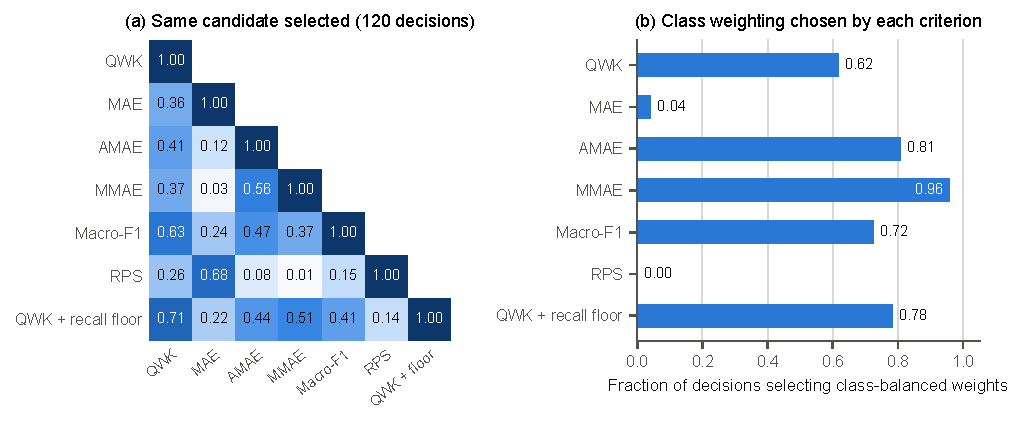
\includegraphics[width=\textwidth]{figures/fig3_agreement_weighting.pdf}
\caption{(a) Fraction of the \NDecisions{} paired selection decisions (\NPrimary{} primary tasks, two model families, two repeats, three outer folds) in which two criteria selected the same candidate. (b) Fraction of decisions in which each criterion selected the class-balanced version of a candidate.}\label{fig:agree}
\end{figure}

\subsection{No criterion is safe across metrics}\label{sec:res-regret}

Figure~\ref{fig:regret} shows the normalized regret of each criterion on each evaluation metric. On its own metric every criterion was close to the best single candidate (diagonal regret at most \RegOwnMax{}), but each paid elsewhere. The criteria favoured by aggregate error had a large endpoint regret (MAE \RegEndMae{}, RPS \RegEndRps{}), and those favoured by endpoint performance paid on MAE (MMAE \RegMaeMmae{}, \QWKF{} \RegMaeCon{}). QWK, macro-F1 and AMAE had an endpoint regret of \RegEndQwk{}, \RegEndMfone{} and \RegEndAmae{}, about halfway between the best and the worst candidate. \QWKF{} (\RegEndCon{}) and MMAE (\RegEndMmae{}) had the lowest endpoint regret.

Friedman tests with the \FriedBlocks{} sources as blocks (Table~S5 in Online Resource~1) agree with this pattern but have little power. For endpoint recall the criteria differed ($\chi^2_6=\FriedEndChi$, $p\FriedEndP$): \QWKF{} (mean rank \RankEndCon{}) and MMAE (\RankEndMmae{}) ranked best, QWK, macro-F1 and AMAE lay in the middle (\RankEndQwk{}, \RankEndMfone{} and \RankEndAmae{}), and MAE (\RankEndMae{}) and RPS (\RankEndRps{}) ranked worst. With nine blocks the Nemenyi critical difference is \NemenyiCD{}, larger than the largest difference in mean ranks (\FriedEndMaxDiff{}), so no pair of criteria was separated. For QWK itself the ranking differed, with QWK first (\RankQwkQwk{}), \QWKF{} second (\RankQwkCon{}) and MMAE last (\RankQwkMmae{}), but the criteria did not differ significantly ($\chi^2_6=\FriedQwkChi$, $p\FriedQwkP$).

\begin{figure}[t]
\centering
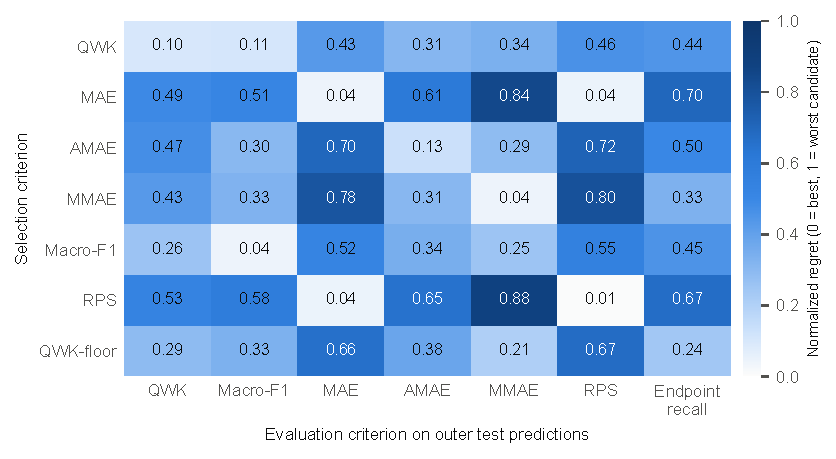
\includegraphics[width=0.85\textwidth]{figures/fig2_regret_matrix.pdf}
\caption{Normalized cross-criterion regret on outer test predictions, averaged over the \NCells{} primary task--family cells and two repeats. Rows: criterion used for selection; columns: metric used for evaluation. 0 corresponds to the best and 1 to the worst of the four candidates in the family, identified retrospectively.}\label{fig:regret}
\end{figure}

\subsection{Endpoint recall: what changes relative to QWK}\label{sec:res-endpoint}

Table~\ref{tab:endpoint} and Fig.~\ref{fig:endpoint} report the endpoint contrasts. Under QWK selection several cells had low endpoint recall, notably in the wine tasks, where the QWK-selected models almost never predicted the extreme scores (for PO, QWK selected the unweighted candidates in every decision). The AMAE$-$QWK difference ranged from \AmaeMin{} (MovieLens-100k, PO) to \AmaeMax{} (red wine, PO) and changed sign across tasks; averaged over the two families, it was positive in \WilPosAmae{} and negative in \WilNegAmae{} of the \NBlocks{} sources (Table~\ref{tab:inference}; median \WilMedAmae{}, $p=\WilPAmae$). Macro-F1 differed from QWK in both directions (\WilPosMfone{} increases, \WilNegMfone{} decreases). In this pool \QWKF{} never reduced $R_{\mathrm{end}}$ in any task--family cell (but see Section~\ref{sec:res-stage4}): averaged over the families, it increased it in \WilPosCon{} of the \NBlocks{} sources and left it unchanged in the other \ConZero{} (median \WilMedCon{}, mean \WilMeanCon{}; exact $p=\WilPCon$, Holm-adjusted $p=\HolmCon$). By construction, it departs from QWK only when the QWK-selected candidate violates the floor on the inner predictions. Where its effect on QWK was nonzero, QWK was lower in \QwkCostNegCon{} sources and higher in \QwkCostPosCon{}, and the largest QWK loss in any task--family cell was \ConQwkCostMaxAbs{}. The floor was often infeasible on the inner predictions of the wine tasks, which have very few endpoint cases; \ConFallbacksWine{} of the \ConFallbacks{} fallbacks to AMAE occurred there. MMAE increased endpoint recall in \WilPosMmae{} and decreased it in \WilNegMmae{} sources ($p=\WilPMmae$), while MAE and RPS reduced endpoint recall relative to QWK in \WilNegMae{} and \WilNegRps{} sources, respectively ($p=\WilPMae$ and $p=\WilPRps$). Every criterion other than \QWKF{} lowered QWK in most sources (Table~\ref{tab:inference}), as expected when QWK is the reference. None of the three primary contrasts was significant after Holm's correction, either within a model family or with the families averaged; with nine sources these tests have little power.

\begin{table}[t]
\caption{Endpoint recall under QWK selection ($R_0$, $R_{K-1}$) and differences in mean endpoint recall $R_{\mathrm{end}}$ relative to QWK selection, with 95\% paired group-bootstrap intervals conditional on the fitted models. Last column: change in QWK caused by the recall floor. PO: proportional odds; RF: random forest.}\label{tab:endpoint}
\centering\scriptsize
\setlength{\tabcolsep}{3pt}
\begin{tabular}{@{}llcccccc@{}}
\toprule
& & \multicolumn{2}{c}{QWK selection} & \multicolumn{3}{c}{$\Delta R_{\mathrm{end}}$ relative to QWK} & $\Delta$QWK\\
\cmidrule(lr){3-4}\cmidrule(lr){5-7}
Task & Family & $R_0$ & $R_{K-1}$ & AMAE & MMAE & \QWKF{} & \QWKF{}\\
\midrule
Wine (red) & PO & 0.00 & 0.00 & \ensuremath{+}0.53 [\ensuremath{+}0.33, \ensuremath{+}0.73] & \ensuremath{+}0.53 [\ensuremath{+}0.33, \ensuremath{+}0.73] & \ensuremath{+}0.53 [\ensuremath{+}0.33, \ensuremath{+}0.75] & \ensuremath{-}0.031 \\
 & RF & 0.00 & 0.06 & \ensuremath{+}0.11 [\ensuremath{+}0.03, \ensuremath{+}0.20] & \ensuremath{+}0.11 [\ensuremath{+}0.03, \ensuremath{+}0.21] & \ensuremath{+}0.11 [\ensuremath{+}0.03, \ensuremath{+}0.20] & \ensuremath{-}0.056 \\
Wine (white) & PO & 0.00 & 0.00 & \ensuremath{+}0.10 [\ensuremath{+}0.01, \ensuremath{+}0.23] & \ensuremath{+}0.04 [0.00, \ensuremath{+}0.08] & \ensuremath{+}0.39 [\ensuremath{+}0.22, \ensuremath{+}0.58] & \ensuremath{-}0.032 \\
 & RF & 0.07 & 0.00 & 0.00 [0.00, 0.00] & \ensuremath{+}0.06 [0.00, \ensuremath{+}0.18] & 0.00 [0.00, 0.00] & 0.000 \\
SkillCraft & PO & 0.56 & 0.70 & 0.00 [\ensuremath{-}0.01, 0.00] & 0.00 [0.00, 0.00] & 0.00 [0.00, 0.00] & 0.000 \\
 & RF & 0.46 & 0.14 & \ensuremath{+}0.19 [\ensuremath{+}0.13, \ensuremath{+}0.24] & 0.00 [0.00, 0.00] & \ensuremath{+}0.25 [\ensuremath{+}0.18, \ensuremath{+}0.32] & \ensuremath{-}0.023 \\
Restaurant & PO & 0.17 & 0.58 & \ensuremath{-}0.01 [\ensuremath{-}0.03, \ensuremath{+}0.01] & \ensuremath{+}0.05 [\ensuremath{+}0.01, \ensuremath{+}0.09] & \ensuremath{+}0.05 [0.00, \ensuremath{+}0.09] & \ensuremath{-}0.029 \\
 & RF & 0.13 & 0.63 & \ensuremath{-}0.01 [\ensuremath{-}0.02, \ensuremath{+}0.01] & 0.00 [\ensuremath{-}0.04, \ensuremath{+}0.05] & 0.00 [\ensuremath{-}0.04, \ensuremath{+}0.04] & \ensuremath{-}0.033 \\
Sushi & PO & 0.45 & 0.45 & 0.00 [0.00, 0.00] & 0.00 [0.00, 0.00] & 0.00 [0.00, 0.00] & 0.000 \\
 & RF & 0.33 & 0.32 & 0.00 [\ensuremath{-}0.01, 0.00] & 0.00 [\ensuremath{-}0.01, 0.00] & 0.00 [0.00, 0.00] & 0.000 \\
MovieLens-100k & PO & 0.52 & 0.40 & \ensuremath{-}0.40 [\ensuremath{-}0.43, \ensuremath{-}0.38] & 0.00 [0.00, 0.00] & 0.00 [0.00, 0.00] & 0.000 \\
 & RF & 0.26 & 0.38 & \ensuremath{-}0.09 [\ensuremath{-}0.10, \ensuremath{-}0.08] & \ensuremath{+}0.08 [\ensuremath{+}0.05, \ensuremath{+}0.11] & \ensuremath{+}0.05 [\ensuremath{+}0.03, \ensuremath{+}0.07] & \ensuremath{-}0.017 \\

\bottomrule
\end{tabular}
\end{table}

\begin{table}[t]
\caption{Cross-task summary of differences relative to QWK selection over the \NBlocks{} primary sources (the two wine tasks form one source). $+/-$: number of sources with a positive or negative difference in $R_{\mathrm{end}}$ (zeros omitted) for proportional odds (PO), random forest (RF) and both families averaged within each source (Both). Median, exact Wilcoxon $p$ and Holm-adjusted $p$ (three primary contrasts) refer to Both, as do the sign counts and median of the QWK difference in the last two columns.}\label{tab:inference}
\centering\footnotesize
\begin{tabular}{@{}lcccrrrcr@{}}
\toprule
& \multicolumn{6}{c}{$\Delta R_{\mathrm{end}}$} & \multicolumn{2}{c}{$\Delta$QWK}\\
\cmidrule(lr){2-7}\cmidrule(lr){8-9}
Contrast & PO $+/-$ & RF $+/-$ & Both $+/-$ & Median & $p$ & Holm $p$ & $+/-$ & Median\\
\midrule
AMAE $-$ QWK & 3/5 & 4/5 & 7/10 & \ensuremath{-}0.003 & 0.611 & 1.000 & 3/14 & \ensuremath{-}0.015 \\
Macro-F1 $-$ QWK & 5/2 & 3/5 & 8/7 & 0.000 & 0.847 & 1.000 & 2/14 & \ensuremath{-}0.003 \\
QWK+floor $-$ QWK & 3/0 & 5/0 & 8/0 & 0.000 & 0.008 & 0.023 & 2/6 & 0.000 \\
MMAE $-$ QWK & 6/2 & 5/3 & 11/5 & \ensuremath{+}0.002 & 0.433 & -- & 2/15 & \ensuremath{-}0.017 \\
MAE $-$ QWK & 1/6 & 2/5 & 3/11 & \ensuremath{-}0.017 & 0.035 & -- & 3/13 & \ensuremath{-}0.017 \\
RPS $-$ QWK & 1/7 & 3/5 & 4/12 & \ensuremath{-}0.028 & 0.044 & -- & 4/13 & \ensuremath{-}0.020 \\

\bottomrule
\end{tabular}
\end{table}

\begin{figure}[t]
\centering
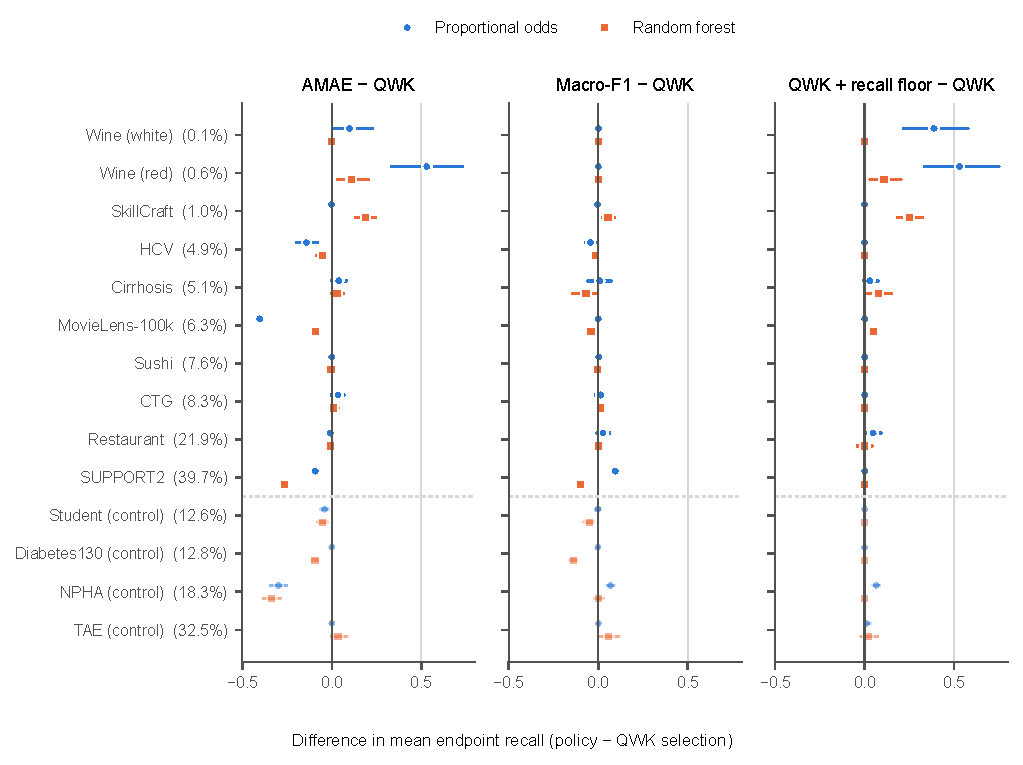
\includegraphics[width=\textwidth]{figures/fig1_endpoint_contrasts.pdf}
\caption{Differences in mean endpoint recall between three criteria and QWK selection, with 95\% paired group-bootstrap intervals conditional on the fitted models. Within the primary and the control block, tasks are ordered by the share of the rarer endpoint category (in parentheses). Control tasks are below the dashed line.}\label{fig:endpoint}
\end{figure}

\subsection{Why the weighting choice follows the criterion}\label{sec:res-weights}

The fixed-hyperparameter controls (Table~\ref{tab:controls}) support Remark~\ref{rem:weights}. Balanced weights increased normalized MAE in \CtrlPosMae{} of the \CtrlN{} comparisons (median \CtrlMedMae{}) but decreased normalized MMAE in \CtrlNegMmae{} (median \CtrlMedMmae{}); mean endpoint recall increased in \CtrlPosEnd{} (median \CtrlMedEnd{}) and QWK in \CtrlPosQwk{}. A criterion built on aggregate error (MAE, RPS) therefore sees weighting as almost uniformly harmful, and a criterion built on the worst category (MMAE) sees it as almost uniformly beneficial, which is the selection behaviour in Fig.~\ref{fig:agree}b.

The effect on each endpoint followed its share (Fig.~\ref{fig:share}a). Weighting increased the recall of every endpoint whose share was below the uniform share $1/K$ (\EpWBelowPos{} of \EpWBelowN{} endpoint--family points; median \EpWBelowMed{}) and decreased it for \EpWAboveNeg{} of the \EpWAboveN{} endpoints above it (median \EpWAboveMed{}); Spearman's $\rho$ between the change and $\log(K\pi_c)$ was \EpWRho{} (task-cluster bootstrap 95\% interval \EpWRhoLo{} to \EpWRhoHi{}), and the share of points that moved in the predicted direction was \EpWAgr{} (\EpWAgrLo{} to \EpWAgrHi{}). Intervals that resample the \NSourcesRule{} sources instead of the tasks were similar (\EpWRhoLoS{} to \EpWRhoHiS{} for $\rho$; Table~S10 in Online Resource~1), here and for the AMAE and stage-4 comparisons below. Proposition~\ref{prop:reweight} held without exception in the weighted training itself: when the endpoint was the rarest category, weighting never reduced its recall (\PcRarestOk{} of \PcRarestN{} comparisons of one family and hyperparameter setting), and when it was the most frequent category, weighting never increased it (\PcFreqOk{} of \PcFreqN{}). Applying the prior correction $m_c=1/(K\pi_c)$ to the outer probabilities of the unweighted candidates reproduced the direction of the actual weighting effect in \PcAgreePct{}\% of the \PcAgreeN{} comparisons in which both changes were nonzero. Endpoints above $1/K$ were common: the normal fetal state in CTG, blood donors in HCV, both endpoints of SUPPORT2 and the upper endpoints of Restaurant and Sushi. In the four third-stage tasks, which were added after the first two stages had been analysed, \SThreeWCons{} of the \SThreeWN{} endpoint--family points changed in the direction given by the rule.

\begin{table}[t]
\caption{Fixed-hyperparameter controls: balanced minus unweighted training for the same family, hyperparameter, splits and seeds (\NPrimary{} primary tasks $\times$ two families $\times$ two hyperparameter settings = \CtrlN{} comparisons). Counts of increases and decreases, median and range of the differences.}\label{tab:controls}
\centering\footnotesize
\begin{tabular}{@{}lrrrr@{}}
\toprule
Metric & Increase & Decrease & Median & Range\\
\midrule
Lower-endpoint recall & 23 & 0 & \ensuremath{+}0.320 & [0.000, \ensuremath{+}0.519] \\
Upper-endpoint recall & 15 & 8 & \ensuremath{+}0.121 & [\ensuremath{-}0.613, \ensuremath{+}0.700] \\
Mean endpoint recall & 21 & 3 & \ensuremath{+}0.145 & [\ensuremath{-}0.148, \ensuremath{+}0.531] \\
QWK & 17 & 7 & \ensuremath{+}0.020 & [\ensuremath{-}0.043, \ensuremath{+}0.172] \\
Normalized MAE & 24 & 0 & \ensuremath{+}0.083 & [\ensuremath{+}0.007, \ensuremath{+}0.152] \\
Normalized AMAE & 9 & 15 & \ensuremath{-}0.020 & [\ensuremath{-}0.134, \ensuremath{+}0.044] \\
Normalized MMAE & 2 & 22 & \ensuremath{-}0.204 & [\ensuremath{-}0.527, \ensuremath{+}0.071] \\
Share of endpoint predictions & 20 & 4 & \ensuremath{+}0.108 & [\ensuremath{-}0.494, \ensuremath{+}0.691] \\

\bottomrule
\end{tabular}
\end{table}

\subsection{When AMAE helps or hurts the endpoints}\label{sec:res-share}

On these tasks AMAE selection followed the same rule (Fig.~\ref{fig:share}b); on new sources it did not (Section~\ref{sec:res-stage5}). For endpoints below $1/K$, the AMAE-selected model had higher recall than the QWK-selected one for \EpABelowPos{} and lower recall for \EpABelowNeg{} of the \EpABelowN{} points (median \EpABelowMed{}); for endpoints above $1/K$ it had lower recall for \EpAAboveNeg{} of \EpAAboveN{} (median \EpAAboveMed{}); $\rho=\EpARho$ (task-cluster bootstrap 95\% interval \EpARhoLo{} to \EpARhoHi{}). In the third-stage tasks, \SThreeACons{} of the \SThreeANonzero{} nonzero changes had the predicted sign. This explains why the AMAE$-$QWK contrast in mean endpoint recall changed sign across tasks: it is positive when both endpoints are rare, as in the wine tasks and SkillCraft, and negative when an endpoint is the majority category or when AMAE drifts towards the middle category (Section~\ref{sec:res-constant}). At the task level, the same pattern appears as a correlation between the AMAE$-$QWK difference and the share of the rarer endpoint ($\rho=\ModRho{}$ over \ModCells{} cells), but the per-endpoint view is more informative because a single task can have one endpoint below and one above $1/K$.

\begin{figure}[t]
\centering
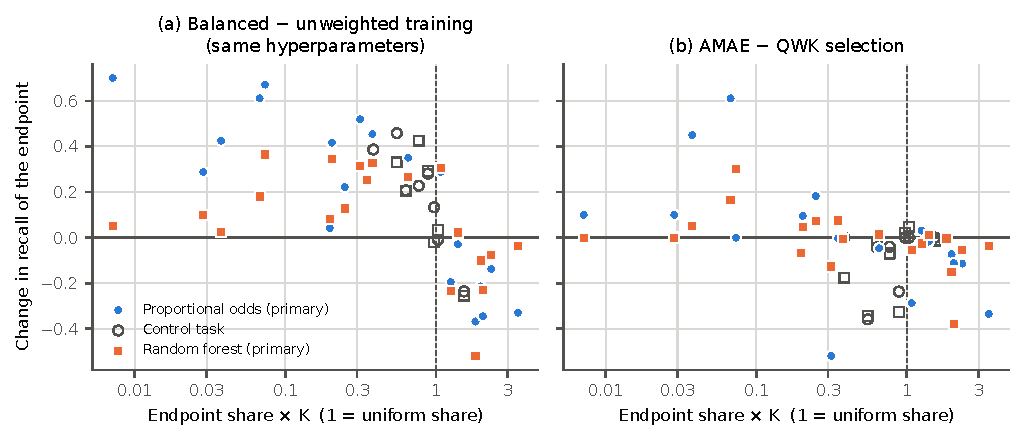
\includegraphics[width=\textwidth]{figures/fig4_endpoint_share.pdf}
\caption{Change in the recall of each endpoint category against its share relative to the uniform share ($K\pi_c$, log scale; dashed line: $K\pi_c=1$). (a) Balanced minus unweighted training at fixed hyperparameters (mean of the two settings). (b) AMAE-selected minus QWK-selected model. Filled markers: primary tasks; open markers: control tasks.}\label{fig:share}
\end{figure}

\subsection{AMAE and the constant-prediction level}\label{sec:res-constant}

Table~\ref{tab:constant} compares the candidates with the no-information level $\nu_K$ of Proposition~\ref{prop:constant}. In \NConstWorseTasks{} primary tasks (the three rating tasks and SUPPORT2), \emph{all eight} candidates had a higher normalized AMAE than the constant middle-category prediction; for example, in MovieLens-100k $\nu_5=\ConstNamaeMl{}$ against a best candidate value of \BestCandNamaeMl{}, and in SUPPORT2 $\nu_5=\ConstNamaeSp{}$ against \BestCandNamaeSp{}. In these tasks QWK of the selected models ranged from \QwkRangeLow{} to \QwkRangeHigh{}, and within the pool AMAE prefers the candidates closest to the degenerate rule. In the three rating tasks the signal is weak; in SUPPORT2 it is moderate, but the two endpoints are the largest categories, so the equal class weighting of AMAE emphasizes the rare middle categories (Section~\ref{sec:res-share}). MovieLens-100k with PO is the clearest case. The QWK-selected model (balanced weights) spread its predictions widely: prediction variance \PredVarMlPoQwk{} against a label variance of \LabVarMl{}, and \EndShareMlPoQwk{} of predictions in an endpoint category against a true share of \LabEndMl{}. It reached $R_0=\LowMlPoQwk{}$ and $R_{K-1}=\HighMlPoQwk{}$. The AMAE-selected model (no weights) concentrated its predictions in the middle (variance \PredVarMlPoAmae{}, endpoint share \EndShareMlPoAmae{}), had $R_0=\LowMlPoAmae{}$ and $R_{K-1}=\HighMlPoAmae{}$, and a worse normalized MMAE (\NmmaeMlPoAmae{} against \NmmaeMlPoQwk{}), although its normalized AMAE was lower (\NamaeMlPoAmae{} against \NamaeMlPoQwk{}). In QWK terms the dispersed model had a larger observed disagreement ($O=\ObsMlPoQwk{}$ against \ObsMlPoAmae{}) but an even larger expected disagreement ($E=\ExpMlPoQwk{}$ against \ExpMlPoAmae{}), as described in Remark~\ref{rem:qwk}. The control task NPHA, with QWK between \NphaQwkLow{} and \NphaQwkHigh{} and \NphaConstWorse{} of eight candidates above $\nu_3$, showed the same pattern (AMAE$-$QWK: \NphaAmaePo{} for PO and \NphaAmaeRf{} for RF).

The direction reversed where the endpoints were very rare. In red wine with PO, QWK selected an unweighted model that predicted almost only middle scores (prediction variance \PredVarWrPoQwk{}, label variance \LabVarWr{}; endpoint share \EndShareWrPoQwk{}, true share \LabEndWr{}), whereas AMAE selected the balanced model (variance \PredVarWrPoAmae{}, endpoint share \EndShareWrPoAmae{}), with $R_0=\LowWrPoAmae{}$ and $R_{K-1}=\HighWrPoAmae{}$. Neither criterion has a fixed preference for concentrated or dispersed predictions; which one protects the endpoints depends on the class shares and on the signal in the task.

\begin{table}[t]
\caption{Normalized AMAE of the constant middle-category prediction ($\nu_K$, Proposition~\ref{prop:constant}) compared with the best candidate, the QWK-selected and the AMAE-selected models (PO / RF), the number of candidates worse than the constant rule, and QWK of the QWK-selected models (PO / RF).}\label{tab:constant}
\centering\footnotesize
\begin{tabular}{@{}lrrrcccc@{}}
\toprule
Task & $K$ & $\nu_K$ & Best cand. & QWK-sel. & AMAE-sel. & Worse than $\nu_K$ & QWK of QWK-sel.\\
\midrule
Wine (red) & 6 & 0.300 & 0.153 & 0.212 / 0.173 & 0.154 / 0.168 & 0/8 & 0.50 / 0.54 \\
Wine (white) & 7 & 0.286 & 0.193 & 0.226 / 0.193 & 0.236 / 0.193 & 0/8 & 0.40 / 0.55 \\
SkillCraft & 7 & 0.286 & 0.124 & 0.124 / 0.131 & 0.124 / 0.132 & 0/8 & 0.73 / 0.73 \\
Restaurant & 3 & 0.333 & 0.407 & 0.424 / 0.420 & 0.414 / 0.422 & 8/8 & 0.08 / 0.07 \\
Sushi & 5 & 0.300 & 0.336 & 0.377 / 0.344 & 0.377 / 0.339 & 8/8 & 0.18 / 0.16 \\
MovieLens-100k & 5 & 0.300 & 0.320 & 0.354 / 0.326 & 0.323 / 0.321 & 8/8 & 0.20 / 0.21 \\
\midrule
TAE (control) & 3 & 0.333 & 0.328 & 0.340 / 0.390 & 0.340 / 0.389 & 7/8 & 0.29 / 0.22 \\

\bottomrule
\end{tabular}
\end{table}

\subsection{Controlled simulation}\label{sec:res-sim}

Under the latent Gaussian model the AMAE$-$QWK differences in $R_{\mathrm{end}}$ were small: \SimAmaeAbsSmall{} of the \SimCells{} prior--signal--family cells had an absolute difference below 0.02, and the range was \SimAmaeMin{} to \SimAmaeMax{} (Table~S4 in Online Resource~1). The largest effects occurred for random forests with rare endpoints, with opposite signs at low and high signal. At high signal the per-endpoint changes agreed with the endpoint-share rule: with the asymmetric prior and PO, the endpoint with share 0.45 lost recall (\SimAsymPoLow{}) and the endpoint with share 0.05 gained (\SimAsymPoHigh{}); with the symmetric rare prior and RF both rare endpoints gained (\SimSymHiRfLow{} and \SimSymHiRfHigh{}). At low signal the same RF cell lost recall in both endpoints (\SimSymLoRfLow{} and \SimSymLoRfHigh{}). The simulation therefore supports the rule only when the candidates carry enough signal, and it does not reproduce the size of the largest real-data contrasts, which arose where very unequal class shares, weak signal and imperfect candidate models occurred together. It was not designed to establish such a mechanism.

\subsection{Control and superseded tasks}

In the control tasks the criteria behaved as in the primary tasks (Fig.~\ref{fig:endpoint}): \QWKF{} never reduced endpoint recall, AMAE reduced it most in the low-signal NPHA task, and in TAE, whose three categories are nearly balanced, no criterion reduced endpoint recall relative to QWK. In the superseded eight-league SkillCraft task, AMAE selection with RF raised endpoint recall relative to QWK, in the same direction as the seven-league task but with a smaller effect (Table~S2 in Online Resource~1).

\subsection{Pre-specified robustness stage}\label{sec:res-stage4}

Table~\ref{tab:stage4} lists the stage-4 predictions and their outcomes: four of the five predictions for the expanded pool and two of the three for the simulation were supported. With 24 candidates from three families the criteria disagreed as before (QWK and AMAE selected the same candidate in \HfAgrQwkAmae{} of the \DecFour{} decisions, QWK and \QWKF{} in \HfAgrQwkCon{}), and the criterion again decided the weighting (H1): MAE and RPS selected balanced weights in \BalFourMae{} and \BalFourRps{} of their decisions and MMAE in \BalFourMmae{}, with the same ordering in each family (Table~S6 in Online Resource~1). The endpoint-share rule held for weighting (H2; Fig.~\ref{fig:stage4}a): the proportion of points with the predicted sign was \HfWAgr{} (task-cluster 95\% interval \HfWAgrLo{} to \HfWAgrHi{}) and $\rho=\HfWRho$ (\HfWRhoLo{} to \HfWRhoHi{}). Apart from two zero changes (gradient boosting never predicted the rarest wine score, with or without weights), the \HfWExcN{} exceptions were endpoints just above the boundary, with $K\pi_c$ between \HfWExcLo{} and \HfWExcHi{}. It also held for AMAE selection (H3; Fig.~\ref{fig:stage4}b): agreement \HfAAgr{} (\HfAAgrLo{} to \HfAAgrHi{}) over the \HfANonzero{} nonzero points and $\rho=\HfARho$ (\HfARhoLo{} to \HfARhoHi{}); the largest exceptions were the lowest category of MovieLens-100k in all three families, where AMAE again preferred models close to the constant rule. The AMAE$-$QWK difference in $R_{\mathrm{end}}$ ranged from \HfAmaeMin{} to \HfAmaeMax{}, and in the same \HfConstTasks{} tasks as before (\HfConstTaskList{}) all 24 candidates had a higher normalized AMAE than the constant middle-category prediction. Every criterion had a regret of at least \HfRegMinMax{} on some other metric (H5; Table~S7 in Online Resource~1).

H4 was not supported. The recall floor lowered $R_{\mathrm{end}}$ relative to QWK in \HfFloorDec{} of the \HfFloorCells{} task--family cells: by at most \HfFloorSmallMax{} in four of them, and by \HfFloorMinAbs{} for gradient boosting on MovieLens-100k. In that cell the floor departed from the QWK choice in two of six decisions, in both of which no candidate met the floor on the inner predictions; the fallback to AMAE then selected unweighted candidates whose recall of the lowest category on the outer folds was below 0.05. Meeting the floor on the inner predictions does not guarantee it on the outer folds: in the \FloorFeasCells{} cells in which every departure from QWK met the floor on the inner predictions, $R_{\mathrm{end}}$ fell in \FloorFeasNeg{}, by at most \FloorFeasMaxLoss{} (\FloorFeasWorstTask{}). When the floor cannot be met, the fallback decides, and an AMAE fallback inherits the weakness described in Section~\ref{sec:res-constant}.

In the simulation (Fig.~\ref{fig:stage4}c,d; Table~S8 in Online Resource~1), weighting changed the recall of the lowest category with the predicted sign at every share level, in both families and at all three signal levels, so S1 was supported, and the change decreased with $\pi_0$ (S2; $\rho$ between \SfTwoMin{} and \SfTwoMax{}). At $K\pi_0=1$ the mean change was at most \SfKOneMax{} in absolute value and every Monte Carlo interval contained zero, as the rule implies. S3 was not supported. At $\lambda=2$ the AMAE$-$QWK difference had the predicted sign wherever it was nonzero, but at $\lambda=1$ it was negative for $\pi_0=0.10$ in both families (\SfThreePo{} for PO and \SfThreeRf{} for RF, with intervals including zero), and at $\lambda=0.5$, for which no prediction was made, AMAE selection lowered the recall of the lowest category for every $\pi_0\le0.10$ (from \SfLowSigAmin{} to \SfLowSigAmax{}) although weighting itself raised it. The effect of weighting on an endpoint is therefore a robust consequence of its share, whereas the effect of AMAE selection also depends on the signal: with weak signal, AMAE tends towards the constant middle-category rule and away from the rare endpoints.

\begin{table}[t]
\caption{Pre-specified predictions of stage 4 and their outcomes. H1--H5: expanded pool of 24 candidates, primary tasks; brackets give task-cluster bootstrap 95\% intervals. S1--S3: simulation, lowest category, $\lambda\in\{1,2\}$; $\Delta_w$: balanced minus unweighted recall; $\Delta_a$: AMAE-selected minus QWK-selected recall.}\label{tab:stage4}
\centering\footnotesize
\begin{tabular}{@{}lp{5.2cm}p{4.3cm}l@{}}
\toprule
& Prediction & Result & Supported\\
\midrule
H1 & Balanced weights chosen in $<0.20$ of decisions by MAE and RPS, $>0.80$ by MMAE; MAE and RPS below MMAE in every family & MAE 0.04, RPS 0.01, MMAE 0.93 & Yes\\
H2 & Weighting raises endpoints with $K\pi<1$ and lowers those with $K\pi>1$: agreement interval above 0.5, $\rho$ interval below 0 & agreement 0.90 [0.80, 0.98]; $\rho=\ensuremath{-}0.60$ [\ensuremath{-}0.75, \ensuremath{-}0.26] & Yes\\
H3 & As H2 for AMAE$-$QWK selection (zeros excluded from agreement) & agreement 0.81 [0.67, 0.93]; $\rho=\ensuremath{-}0.62$ [\ensuremath{-}0.78, \ensuremath{-}0.30]; 13 zeros & Yes\\
H4 & \QWKF{}$-$QWK in $R_{\mathrm{end}}\ge-0.02$ in every task--family cell & minimum \ensuremath{-}0.081; 5 decreases, 7 increases in 30 cells & \textbf{No}\\
H5 & Every criterion has regret $\ge0.30$ on some other metric & smallest maximum 0.48 (QWK) & Yes\\
\midrule
S1 & $\Delta_w>0$ for $\pi_0\le0.10$ and $<0$ for $\pi_0\ge0.30$ ($\lambda\in\{1,2\}$, each family) & 4 of 4 family--signal cells & Yes\\
S2 & Spearman $\rho(\Delta_w,\pi_0)<0$ & $\rho$ from \ensuremath{-}1.00 to \ensuremath{-}0.83 & Yes\\
S3 & Same sign pattern for $\Delta_a$ where nonzero & 2 of 4 family--signal cells & \textbf{No}\\

\bottomrule
\end{tabular}
\end{table}

\begin{figure}[t]
\centering
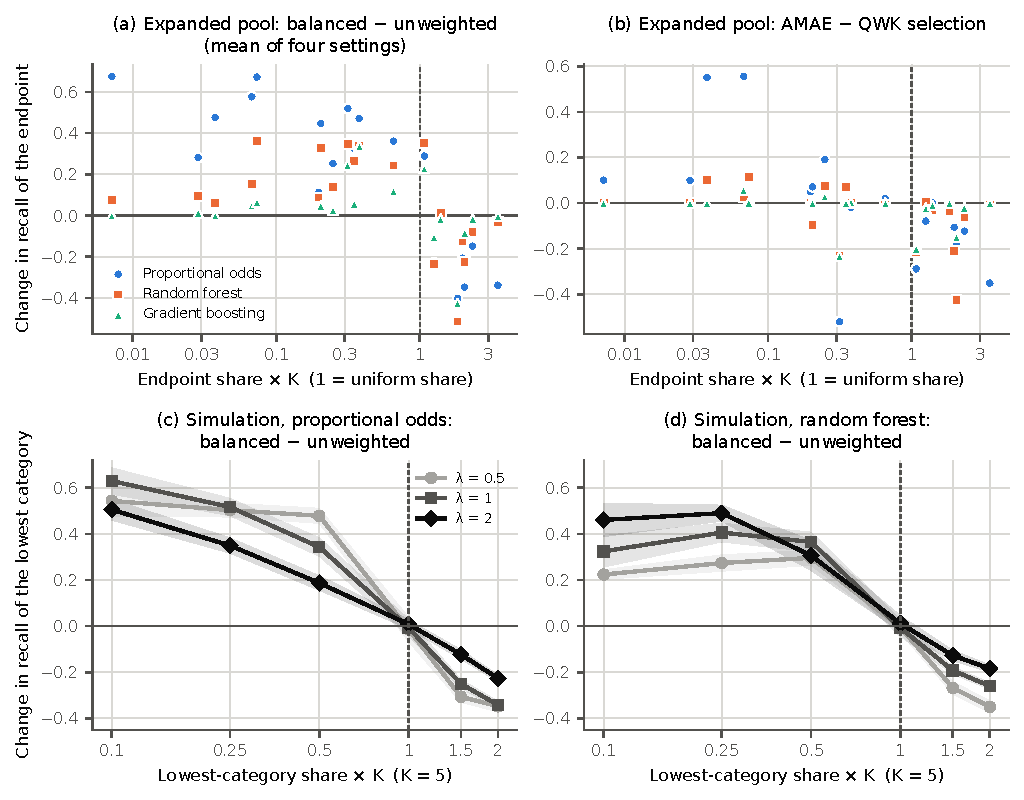
\includegraphics[width=\textwidth]{figures/fig5_stage4_robustness.pdf}
\caption{Stage 4. (a, b) Expanded pool of 24 candidates, primary tasks: change in the recall of each endpoint category against its share relative to the uniform share ($K\pi_c$, log scale), for balanced minus unweighted training (mean over the four hyperparameter settings of a family) and for the AMAE-selected minus the QWK-selected model. (c, d) Simulation: balanced minus unweighted recall of the lowest category against $K\pi_0$ for three signal levels; mean of ten replications with Monte Carlo 95\% intervals. Dashed lines: $K\pi=1$.}\label{fig:stage4}
\end{figure}

\subsection{Pre-registered validation stage}\label{sec:res-stage5}

Table~\ref{tab:stage5} lists the stage-5 predictions: eight of the ten were supported. All \FitsStageFive{} fits completed. The new sources differed in signal (best QWK from \FiveDrugBestQwk{} for alcohol use to above 0.5 for the entrance examination and the NHIS; Table~S9 in Online Resource~1).

\paragraph{New sources.} The criterion again decided the weighting (V1): MAE and RPS never selected balanced weights (\VoneBalMae{} and \VoneBalRps{}) and MMAE always did (\VoneBalMmae{}). The weighting rule met its pre-registered threshold exactly (V2; agreement \VtwoAgr{}, $\rho=\VtwoRho$; Fig.~\ref{fig:stage5}a). The six exceptions came from two endpoints in all three families. One was the excellent-health category of the NHIS, just above the boundary ($K\pi=1.12$). The other was the highest category of alcohol use: its share (\VtwoAlcHighShare\%) is above $1/K$, but its neighbour, use in the last week, is even more frequent (\VtwoAlcNbrShare\%), so weighting moved cases from the neighbour into the endpoint. This is the pairwise logic of Proposition~\ref{prop:reweight}. What matters is an endpoint's share relative to the categories it competes with, which the comparison with $1/K$ only summarizes. Proposition~\ref{prop:reweight} itself held in all \VtwobN{} comparisons in which the endpoint was a rarest category, in all four families (V2b).

The rule for AMAE selection was not supported (V3). In the cells with a QWK of at least 0.30, only \VthreeOk{} of the \VthreeN{} nonzero changes had the predicted sign. On the new sources AMAE selection lowered $R_{\mathrm{end}}$ relative to QWK in \FiveAmaeNeg{} of the \FiveAmaeCells{} task--family cells (differences from \FiveAmaeMin{} to \FiveAmaeMax{}; Fig.~\ref{fig:stage5}b), including endpoints far below $1/K$ in NHANES. In the low-signal alcohol task, \FiveConstDrug{} of the 32 candidates had a higher normalized AMAE than the constant middle-category prediction.

The recall floor with the max--min fallback never lowered $R_{\mathrm{end}}$ on the new sources (V4, \VfourCells{} cells), whereas the AMAE fallback changed it by as much as \VfourOrigMin{}. In the non-blind check on the \VfourOldCells{} cells of the earlier tasks, however, the max--min fallback lost more than 0.02 in two cells (largest change \VfourOldMin{}), where the AMAE fallback had not. Across all \VfourAllCells{} cells, the most negative change was \VfourAllMinStar{} with the max--min fallback and \VfourAllMinOrig{} with the AMAE fallback. Every criterion again had a large regret on some other metric (V5).

\paragraph{Ordinal family and median decoding.} Within the Frank--Hall family, whose selected models reached a QWK similar to gradient boosting (mean \FhQwk{} against \HgbQwk{}), the criterion decided the weighting as before (F1). The weighting rule was not supported (F2). Its agreement interval was above one half (\FtwoAgr{}; \FtwoAgrLo{} to \FtwoAgrHi{}), but the interval for $\rho$ included zero (\FtwoRho{}; \FtwoRhoLo{} to \FtwoRhoHi{}). The three zero changes are wine scores that the family never predicted, and the two other exceptions are endpoints just above $K\pi=1$.

With median decoding, both the weighting rule (D1; agreement \DoneAgr{}, \DoneAgrLo{} to \DoneAgrHi{}; $\rho=\DoneRho$, \DoneRhoLo{} to \DoneRhoHi{}; Fig.~\ref{fig:stage5}c) and the link between criterion and weighting (D2; balanced weights in \DtwoBalMae{} of the MAE and \DtwoBalMmae{} of the MMAE decisions) held, so neither finding is an artefact of argmax decoding.

\paragraph{All primary tasks together.} Over all \PoolWSources{} primary sources, the weighting rule for PO, RF and HGB had an agreement of \PoolWAgr{} (\PoolWAgrLo{} to \PoolWAgrHi{}) and $\rho=\PoolWRho$ (\PoolWRhoLo{} to \PoolWRhoHi{}).

\begin{table}[t]
\caption{Pre-registered predictions of stage 5 and their outcomes. Brackets: source-cluster bootstrap 95\% intervals (for V2 descriptive, with four sources). PO: proportional odds; RF: random forest; HGB: gradient boosting.}\label{tab:stage5}
\centering\footnotesize
\begin{tabular}{@{}lp{5.0cm}p{4.5cm}l@{}}
\toprule
& Prediction & Result & Supported\\
\midrule
\multicolumn{4}{@{}l}{\emph{Part A: four new sources; PO, RF and HGB unless stated}}\\
V1 & Balanced weights chosen in $<0.20$ of decisions by MAE and RPS, $>0.80$ by MMAE & MAE 0.00, RPS 0.00, MMAE 1.00 & Yes\\
V2 & Weighting rule: agreement $\ge0.75$ and $\rho<0$ (24 points) & agreement 0.75 [0.50, 1.00]; $\rho=\ensuremath{-}0.22$ [\ensuremath{-}0.55, \ensuremath{-}0.02] & Yes\\
V2b & Implication of Proposition~2 in weighted training: weighting never lowers the recall of a rarest category (four families) & 64 of 64 comparisons & Yes\\
V3 & AMAE rule where QWK of the QWK-selected model $\ge0.30$: agreement $\ge0.75$ & 14 qualifying points; agreement 0.29 & \textbf{No}\\
V4 & Recall floor with max--min fallback: $\Delta R_{\mathrm{end}}\ge-0.02$ in every cell (four families) & minimum 0.000 in 16 cells (AMAE fallback: \ensuremath{-}0.158) & Yes\\
V5 & Every criterion has regret $\ge0.30$ on some other metric & smallest maximum 0.44 (Macro-F1) & Yes\\
\midrule
\multicolumn{4}{@{}l}{\emph{Part B: Frank--Hall ordinal family, all primary tasks}}\\
F1 & As V1 within the ordinal family & MAE 0.10, RPS 0.00, MMAE 0.94 & Yes\\
F2 & Weighting rule; agreement interval above 0.5, $\rho$ interval below 0 & agreement 0.82 [0.62, 1.00]; $\rho=\ensuremath{-}0.36$ [\ensuremath{-}0.69, 0.15] & \textbf{No}\\
\midrule
\multicolumn{4}{@{}l}{\emph{Part C: median decoding, all primary tasks, four families}}\\
D1 & Weighting rule with median-decoded recall & agreement 0.86 [0.73, 0.98]; $\rho=\ensuremath{-}0.55$ [\ensuremath{-}0.77, \ensuremath{-}0.16] & Yes\\
D2 & Selection with median decoding: balanced in $<0.20$ (MAE) and $>0.80$ (MMAE) of decisions & MAE 0.07, MMAE 0.90 & Yes\\

\bottomrule
\end{tabular}
\end{table}

\begin{figure}[t]
\centering
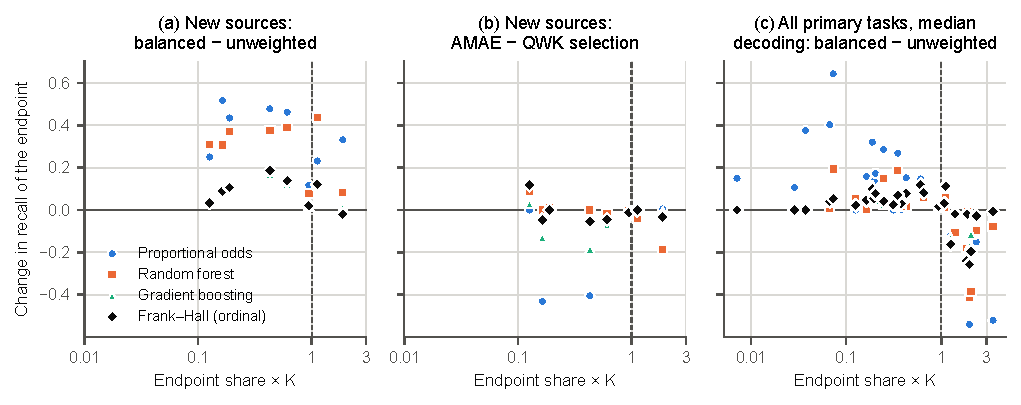
\includegraphics[width=\textwidth]{figures/fig6_stage5_validation.pdf}
\caption{Stage 5. Change in the recall of each endpoint category against its share relative to the uniform share ($K\pi_c$, log scale; dashed line: $K\pi_c=1$). (a) New sources, balanced minus unweighted training (mean over the four settings of a family). (b) New sources, AMAE-selected minus QWK-selected model. (c) All primary tasks, balanced minus unweighted training with median decoding. The pre-registered V2 and V3 use proportional odds, random forest and gradient boosting; the Frank--Hall family is shown for comparison.}\label{fig:stage5}
\end{figure}

%% =====================================================================
\section{Discussion}\label{sec:discussion}

\subsection{Practical implications}

Four recommendations follow. First, the selection criterion should be chosen together with, and reported alongside, the class-weighting decision, because the criterion largely determines that decision: aggregate-error criteria reject weighting and worst-class criteria adopt it. Second, neither class weighting nor AMAE selection protects the endpoint categories in general. Weighting helps an endpoint whose share is below $1/K$ and tends to hurt one whose share is above $1/K$, which is common: in many ordinal data sets the lowest or highest category is the largest one. Comparing each endpoint's share with $1/K$, and with the share of its neighbouring category, before weighting is a simple check. The effect of AMAE selection is less predictable: it followed the same rule on the original tasks but not on the new sources. Third, if the endpoint categories matter, they should be protected explicitly. In our main pool a recall floor added to QWK never reduced endpoint recall, changed the selected model only when the QWK choice violated the floor, and cost at most \ConQwkCostMaxAbs{} in QWK in any task--family cell. A floor met on the inner predictions is not a guarantee for new data, but with 24 candidates the losses in such cells were at most \FloorFeasMaxLoss{}. When the floor cannot be met on the inner predictions, the fallback decides. An AMAE fallback lost up to \VfourAllMinOrigAbs{} in endpoint recall. A fallback to the candidate with the largest smaller endpoint recall avoided these losses on the new sources, but still lost up to \VfourOldMinAbs{} in two earlier cells. How often the floor is infeasible should therefore be reported together with the fallback rule. Fourth, AMAE should be read against its no-information level $\nu_K$ (Proposition~\ref{prop:constant}). Values near $\nu_K$ are compatible with a constant middle-category rule that never predicts an endpoint; in low-signal tasks, minimizing AMAE can favour candidates that drift towards that rule.

These findings complement the binary-classification study of \citet{delaCruzHuayanay2024}, in which some metrics consistently selected good models under simulation. In the ordinal setting studied here no single criterion was close to optimal on all metrics, and the choice is a trade-off that should be made explicit. Relative to earlier ordinal work that tuned models with different metrics \citep{Binotto2025} or pointed to the optimized measure as a possible source of differences between ordinal methods \citep{Buczak2025}, our results add the interaction with class weighting, the endpoint-share rule, the explicit recall floor and the constant-prediction reference for AMAE. Selecting on pooled inner predictions and evaluating on untouched outer folds avoids the optimistic bias of selecting and evaluating on the same data \citep{Varma2006,Cawley2010}; the regret analysis, which looks at the test data, is reported only descriptively.

The two confirmatory stages separate the robust findings from the conditional ones. Three findings held throughout. The link between criterion and weighting held with three times as many candidates, a third model family, four new sources, an ordinal family and median decoding. The endpoint-share rule for weighting held on the new sources, if only at the pre-registered threshold, and in a simulation in which only the share of one category varied the weighting effect changed sign at $K\pi=1$. Proposition~\ref{prop:reweight} held without exception in weighted training. The exceptions to the weighting rule were endpoints close to $K\pi=1$ or next to an even larger category, where the comparison with $1/K$ is too coarse. The rule for AMAE selection did not transfer. It held on the original tasks, in the simulation only with enough signal, and not on the new sources, where AMAE mostly lowered endpoint recall. AMAE should therefore not be used as an indirect way to protect the endpoints. The recall floor is a safeguard whose behaviour depends on its feasibility and its fallback.

\subsection{Limitations}

The evidence is limited in several respects. There are \NPrimary{} primary tasks from \NFamiliesPrimary{} sources, several of them low-signal, three rating tasks with a shared item pool, and some endpoint categories with very few cases. The main candidate pool is deliberately small: two families, two hyperparameter settings each and two weighting options. The larger pools of stages 4 and 5 (up to 32 candidates in four families, including an ordinal decomposition) reproduced the main patterns. Neural and ordinal-forest models, wider grids and joint tuning of weights and decision thresholds were not studied. Apart from the median-decoding check, all criteria use argmax decoding; other criterion-specific decoding rules \citep{Delgado2026} were not studied. Two repeats of three-fold cross-validation and group bootstrap intervals conditional on fitted models do not capture all sources of uncertainty, and the cross-task tests have limited power. The first three stages had locally frozen but not externally registered protocols, and the later stages were designed with knowledge of earlier results; the endpoint-share rule was formulated as a check of Remark~\ref{rem:weights} after the first stages. Stage 4 tested it with pre-specified predictions on the same tasks, under a locally frozen protocol. Stage 5 used new sources and a protocol pushed to a public repository before any fit, but this is not an entry in a registry. Only four new sources passed the eligibility rules, so its V2 decision rested on point estimates. Two of its sources measure the same construct (self-rated health), and survey weights were not used. SkillCraft relies on the source's one-replay-per-participant design, HCV mixes blood donors and patients by design, and the clinical and survey tasks are used only methodologically. Studies with more sources, registered externally, would strengthen the generalization.

%% =====================================================================
\section{Conclusion}\label{sec:conclusion}

In tabular ordinal classification, the criterion used for model selection is not a neutral detail. Within one fixed candidate pool it determined whether class weighting was used, it changed the selected model in most paired decisions, and it changed endpoint recall by up to about 0.5 in either direction relative to QWK. Class weighting helped endpoint categories whose share was below $1/K$ and hurt those above it, AMAE could prefer models close to an uninformative constant rule, and an explicit recall floor on QWK protected the endpoints in almost every cell in which it could be met on the inner predictions. Two confirmatory stages, the second pre-registered with new sources, an ordinal model family and median decoding, supported \PredAllOk{} of \PredAllN{} predictions. They also showed the limits: the effect of AMAE selection on the endpoints did not transfer to new sources, and an infeasible floor is only as good as its fallback. Reporting endpoint recall, worst-class error and the class shares together with the selection criterion is a simple step that makes these trade-offs visible.

%% =====================================================================
\backmatter

\bmhead{Supplementary information}
Online Resource~1 (PDF) contains data provenance, feature definitions and grouping for every task, the stage-4 and stage-5 protocols, full per-policy metrics for all tasks (Table~S1), all policy contrasts with bootstrap intervals (Table~S2), all fixed-hyperparameter controls (Table~S3), the simulation results (Table~S4), source-level Friedman ranks for all evaluation metrics (Table~S5), the stage-4 weighting choices, regret matrix and simulation results (Tables~S6--S8), the stage-5 tasks (Table~S9) and source-cluster bootstrap intervals for the endpoint-share rule (Table~S10).

\section*{Statements and Declarations}

\bmhead{Funding} The authors did not receive support from any organization for the submitted work.

\bmhead{Competing interests} The authors have no relevant financial or non-financial interests to disclose.

\bmhead{Ethics approval and consent to participate} This study is a secondary analysis of publicly documented, de-identified data sets; no new data were collected from human participants.

\bmhead{Data availability} The wine, SkillCraft, Restaurant, TAE, CTG, HCV, Cirrhosis, Diabetes130, Student, NPHA (originally released by ICPSR), Drug Consumption and Entrance Examination data are available from the UCI Machine Learning Repository under CC BY 4.0; the NHANES 2017--2018 and NHIS 2019 public-use files are available from the National Center for Health Statistics under its data user agreement; SUPPORT2 is available from the Vanderbilt Department of Biostatistics data repository, which grants permission for use. The Sushi and MovieLens-100k data permit research use but not redistribution and must be obtained from their providers \citep{Kamishima2003,Harper2015}. Scripts that reproduce the task definitions, subsampling and splits from the original files are provided with the code. Aggregate results (all tables and figures) are included in Online Resource~1 and in the code repository.

\bmhead{Code availability} The code for all stages, the protocols and freeze records, and the aggregate results are available at \url{https://github.com/baturyusuf/XAI-thesis-work-1} (directory \texttt{research/ordinal\_selection\_y1}, tag \texttt{compstat-v2}); \texttt{manuscript\_compstat/reproducibility/README.md} describes how every result is regenerated. The stage-5 protocol was pushed in commit \texttt{66e426e} before any stage-5 model was fitted. The proportional-odds estimator, the shared preprocessor and the RPS function are taken from the authors' earlier public repository \url{https://github.com/baturyusuf/employee-performance-with-XAI} (commit \texttt{c7f7729}); the files used and their SHA-256 hashes are listed in \texttt{SOURCE\_MANIFEST.json} and checked before every fit.

\bmhead{Author contributions} Muhammed Yusuf Batur: conceptualization, methodology, software, data curation, formal analysis, investigation, validation, visualization, project administration, writing -- original draft, writing -- review and editing. Mehmet G\"{o}kt\"{u}rk: conceptualization, methodology, formal analysis, investigation, validation, visualization, supervision, project administration, writing -- original draft, writing -- review and editing. Both authors contributed equally to the conceptual development, methodological design, scientific evaluation, interpretation of the results and preparation of the manuscript, and share first authorship. Both authors read and approved the final manuscript.

\bibliography{refs}

\end{document}
